%\documentclass[journal]{IEEEtran}
\documentclass[10pt,journal,cspaper,compsoc]{IEEEtran}

%packages 
\usepackage{etex}
\usepackage{tikz}
\usepackage{xspace}
\usepackage{arabtex}
\usepackage{graphicx}
%\usepackage{caption}
%\usepackage{subcaption}
\usepackage{framed}
\usepackage{array}
\usepackage{graphics}
\usepackage{booktabs}
\usepackage{multirow}
\usepackage{amssymb}
\usepackage{amsmath}
\usepackage{mathabx}
\usepackage{utf8}
\bibliographystyle{plain}
\usepackage{subfigure}
\usepackage{todonotes}
\usepackage{hyperref}
\usetikzlibrary{shapes,arrows}
\usepackage{color,soul}
\usepackage{verbatim}
\usepackage{array}
\usepackage{multicol}

\usepackage{fancyvrb}
\usepackage{relsize}
\usepackage{wasysym}
\usepackage{pbox}

\def\showvrb#1{%
\texttt{\detokenize{#1}}%
}
%%%%%%%%%%%%%%%%%%%%%%
%macros
\def\framework{\textsc{MERF}\xspace}
\newcommand{\itodo}[1]{\todo[inline,color=green]{\tiny #1}}

\newcolumntype{L}[1]{>{\raggedright\let\newline\\\arraybackslash\hspace{0pt}}m{#1}}
\newcolumntype{C}[1]{>{\centering\let\newline\\\arraybackslash\hspace{0pt}}m{#1}}
\newcolumntype{R}[1]{>{\raggedleft\let\newline\\\arraybackslash\hspace{0pt}}m{#1}}

\newcommand{\TinyRL}[1]{{\RL{#1}}}
\newcommand{\cci}[1]{{\small \texttt{#1}}}
%%%%%%%%%%%%%%%%%%%%%%%
%other 
% correct bad hyphenation here
\hyphenation{op-tical net-works semi-conduc-tor}


%%% RL commands
\newcommand{\utfrl}[1]{\setcode{utf8}\RL{#1}\setcode{standard}}
\newcommand{\notrutfrl}[1]{\transfalse\setcode{utf8}\RL{#1}\setcode{standard}\transtrue}
\newcommand{\notrrl}[1]{\transfalse\RL{#1}\transtrue}
\newcommand{\noarrl}[1]{\arabfalse\RL{#1}\arabtrue}

\begin{document}
%
% paper title
% can use linebreaks \\ within to get better formatting as desired
\title{\framework: Morphology-based Entity and Relational Entity Extraction Framework for Arabic}
%~\IEEEmembership{Member,~IEEE,}
\author{Ameen~Jaber,
        Fadi~A.~Zaraket
\IEEEcompsocitemizethanks{\IEEEcompsocthanksitem A. Jaber and F. Zaraket are with the Department
of Electrical and Computer Engineering, American University of Beirut, Beirut,
Lebanon.\protect\\
E-mail: \{aaj15,fz11\}@aub.edu.lb}}

\IEEEcompsoctitleabstractindextext{%
\begin{abstract}
Rule-based techniques and tools to extract {\em entities} and {\em relational entities} from documents allow users to specify desired entities using natural language questions, finite state automata, regular expressions, structured query language statements, or proprietary scripts.  These techniques and tools require expertise in linguistics and programming and lack support of Arabic {\em morphological analysis} which is key to process Arabic text.
In this work, we present \framework; a morphology-based entity and relational entity extraction framework for Arabic text.  \framework provides a friendly interface where the user, with basic knowledge of linguistic features and regular expressions, defines {\em tag types} and interactively associates them with regular expressions defined over Boolean formulae. Boolean formulae range over matches of Arabic morphological features, and synonymity features. Users define relations with tuples of subexpression matches and can associate code actions with subexpressions. \framework computes feature matches, regular expression matches, and constructs entities and relational entities from the user-defined relations. We evaluated our work with several case studies and compared with existing application-specific techniques. The results show that \framework requires shorter development time and effort compared to existing techniques and produces reasonably accurate results within a reasonable overhead in run time.
\end{abstract}

\begin{IEEEkeywords}
Tagging, Arabic, Natural language processing, Morphological analysis, Computational linguistics, Information extraction, Entity, Relational Entity.
\end{IEEEkeywords}}

% make the title area
\maketitle

% For peerreview papers, this IEEEtran command inserts a page break and
% creates the second title. It will be ignored for other modes.
\IEEEpeerreviewmaketitle

\section{Introduction}
\label{sec:introduction}
\IEEEPARstart{C}{\em omputational Linguistics} (CL) is concerned with building 
accurate linguistic computational models. 
{\em Natural Language Processing} (NLP) is concerned with automating the 
understanding of natural language. 
CL and NLP tasks range from simple ones such as spell checking and typing 
error correction to more 
complex tasks including %text summarization, 
{\em named entity recognition} (NER), {\em cross-document analysis}, 
machine translation, 
and {\em relational entity extraction}~\cite{linckels2011natural,ferilli2011natural}.
Entities are elements of text that are of interest to an NLP task. 
Relational entities are elements that connect entities. 
{\em Annotations} relate chunks of text to {\em labels} denoting
semantic values such as entities or relational entities.
We refer to annotations and labels as {\em tags} and {\em tag types}, respectively, 
in the sequel.

Supervised and unsupervised empirical learning techniques tackle NLP and CL tasks. 
They employ machine learning without the need to manually encode the requisite 
knowledge~\cite{soudi2007arabic}. 
Supervised learning techniques require training corpora that are annotated 
with {\em correct} tags to learn a computational model. 
Supervised and unsupervised techniques require reference corpora that are
annotated with correct tags to evaluate the 
accuracy of the technique in terms of metrics such as precision and 
recall~\cite{englishtreebank,arabictreebank,chinesetreebank}. 

Researchers build the required %seed 
training and reference corpora 
either manually, incrementally using learning techniques, or using knowledge-based 
annotation techniques that recognize and extract entities and relational 
entities from text. 
Knowledge-based techniques use linguistic and 
rhetorical domain specific knowledge encoded into sets of rules 
to extract entities and relational entities~\cite{soudi2007arabic}.
While existing annotation, entity, and relational entity 
extraction tools exist
\cite{chiticariu2010systemt% SystemT
,atzmueller2008rule%Textmarker
,urbain2012user%
,settles2011closing% dualist
,mmax2%MMAX
,brat% BRAT
},
most of them lack Arabic language support, and almost all of them
lack Arabic morphological analysis support that is key to Arabic NLP
due to the rich morphological nature of Arabic~\cite{habash2006arabic}. 
Fassieh~\cite{attia2009fassieh} is a {\em commercial} Arabic annotation tool
with morphological analysis support and text factorization. 
Fassieh lacks support for entity and relational entity extraction.

\transtrue
\setcode{utf8}
\setarab
\transfalse
\begin{figure}[tb]
\begin{center}
\relsize{-0.5}
%\renewcommand{\arraystretch}{1.5}% Wider
\resizebox{\columnwidth}{!}{
    \begin{tabular}{|C{10cm}C{8cm}|} 
      \hline
  \begin{tabular}{R{10cm}}
\RL{تقود} \RL{وأنت} $\stackrel{u1}{\framebox[1.2\width]{\RL{الأول}}}$ $\stackrel{p_2}{\framebox[1.2\width]{\RL{التقاطع}}}$ \RL{من} $\stackrel{r_1}{\framebox[1.2\width]{\RL{بالقرب}}}$ $\stackrel{n_1}{\framebox[1.2\width]{\RL{خليفة}}}$ $\stackrel{p_1}{\framebox[1.2\width]{\RL{برج}}}$ \RL{تلاحظ} \RL{ألا} \RL{المستحيل} \RL{من} 
  \\ ~ \\
$\stackrel{r_3}{\framebox[1.2\width]{\RL{فيها}}}$ \RL{تسلك} \RL{التي} $\stackrel{u_2}{\framebox[1.2\width]{\RL{الأولى}}}$ \RL{المرّة} \RL{هذه} \RL{كانت} \RL{وإن} \RL{حتّى} $\stackrel{n_3}{\framebox[1.2\width]{\RL{زايد،}}}$ $\stackrel{n_2}{\framebox[1.2\width]{\RL{الشيخ}}}$ $\stackrel{p_3}{\framebox[1.2\width]{\RL{شارع}}}$ $\stackrel{r_2}{\framebox[1.2\width]{\RL{في}}}$ \RL{سيارتك}
  \\ ~ \\
\RL{العالم.} \RL{في} \RL{الأطول} \RL{يُعد} \RL{الذي}  $\stackrel{p_7}{\framebox[1.2\width]{\RL{المبنى}}}$ \RL{هذا} \RL{من} $\stackrel{r_4}{\framebox[1.2\width]{\RL{مقربة}}}$ \RL{على} $\stackrel{p_6}{\framebox[1.2\width]{\RL{مول}}}$ $\stackrel{p_5}{\framebox[1.2\width]{\RL{دبيّ}}}$ \RL{يقع} $\stackrel{p_4}{\framebox[1.2\width]{\RL{الطريق؛}}}$ \RL{هذا}
  \\ ~ \\
%  \RL{العالم.} \RL{في} \RL{الأطول} \RL{يُعد} \RL{الذي}  
%  \\
  \multicolumn{1}{L{10cm}}{
   \arabfalse \transtrue
   \RL{من المستحيل ألا تلاحظ برج خليفة بالقرب من التقاطع الأول وأنت تقود سيارتك في شارع الشيخ زايد، حتّى وإن كانت هذه المرّة الأولى التي تسلك فيها هذا الطريق؛ يقع دبيّ مول على مقربة من هذا المبنى الذي يُعد الأطول في العالم.}
   \arabtrue \transfalse} 
  \\ ~ \\
  \multicolumn{1}{L{10cm}}{It is impossible not to notice $\stackrel{n1}{\framebox[1.2\width]{Khalifa}}$ $\stackrel{p_1}{\framebox[1.2\width]{Tower}}$ $\stackrel{r_1}{\framebox[1.2\width]{next to}}$ the $\stackrel{u_1}{\framebox[1.2\width]{first}}$ $\stackrel{p_2}{\framebox[1.2\width]{intersection}}$ while you are driving your car $\stackrel{r_2}{\framebox[1.2\width]{on}}$ $\stackrel{n_2}{\framebox[1.2\width]{Sheikh}}$ $\stackrel{n_3}{\framebox[1.2\width]{Zayed}}$ $\stackrel{p_3}{\framebox[1.2\width]{Road}}$, even if this was $\stackrel{u_2}{\framebox[1.2\width]{the first}}$ time that you take this $\stackrel{p_4}{\framebox[1.2\width]{road}}$; $\stackrel{p_5}{\framebox[1.2\width]{Dubai}}$ $\stackrel{p_6}{\framebox[1.2\width]{Mall}}$ is located $\stackrel{r_4}{\framebox[1.2\width]{near}}$ this $\stackrel{p_7}{\framebox[1.2\width]{building}}$, which is the longest in the world.} 
  \end{tabular}
&
\resizebox{0.6\columnwidth}{!}{
  % Graphic for TeX using PGF
% Title: /home/ameen/Desktop/ergraphEx.dia
% Creator: Dia v0.97.1
% CreationDate: Sat Jan 11 03:49:31 2014
% For: ameen
% \usepackage{tikz}
% The following commands are not supported in PSTricks at present
% We define them conditionally, so when they are implemented,
% this pgf file will use them.
\ifx\du\undefined
  \newlength{\du}
\fi
\setlength{\du}{30\unitlength}
\begin{tikzpicture}
\pgftransformxscale{1.000000}
\pgftransformyscale{-1.000000}
\definecolor{dialinecolor}{rgb}{0.000000, 0.000000, 0.000000}
\pgfsetstrokecolor{dialinecolor}
\definecolor{dialinecolor}{rgb}{1.000000, 1.000000, 1.000000}
\pgfsetfillcolor{dialinecolor}
\definecolor{dialinecolor}{rgb}{1.000000, 1.000000, 1.000000}
\pgfsetfillcolor{dialinecolor}
\pgfpathellipse{\pgfpoint{4.324130\du}{10.573360\du}}{\pgfpoint{1.223030\du}{0\du}}{\pgfpoint{0\du}{0.734470\du}}
\pgfusepath{fill}
\pgfsetlinewidth{0.050000\du}
\pgfsetdash{}{0pt}
\pgfsetdash{}{0pt}
\pgfsetmiterjoin
\definecolor{dialinecolor}{rgb}{0.000000, 0.000000, 0.000000}
\pgfsetstrokecolor{dialinecolor}
\pgfpathellipse{\pgfpoint{4.324130\du}{10.573360\du}}{\pgfpoint{1.223030\du}{0\du}}{\pgfpoint{0\du}{0.734470\du}}
\pgfusepath{stroke}
% setfont left to latex
\definecolor{dialinecolor}{rgb}{0.000000, 0.000000, 0.000000}
\pgfsetstrokecolor{dialinecolor}
\node at (4.324130\du,10.465026\du){\RL{دبي مول}};
% setfont left to latex
\definecolor{dialinecolor}{rgb}{0.000000, 0.000000, 0.000000}
\pgfsetstrokecolor{dialinecolor}
\node at (4.324130\du,10.888360\du){Dubai Mall};
\definecolor{dialinecolor}{rgb}{1.000000, 1.000000, 1.000000}
\pgfsetfillcolor{dialinecolor}
\pgfpathellipse{\pgfpoint{6.415976\du}{8.893981\du}}{\pgfpoint{1.395976\du}{0\du}}{\pgfpoint{0\du}{0.720041\du}}
\pgfusepath{fill}
\pgfsetlinewidth{0.050000\du}
\pgfsetdash{}{0pt}
\pgfsetdash{}{0pt}
\pgfsetmiterjoin
\definecolor{dialinecolor}{rgb}{0.000000, 0.000000, 0.000000}
\pgfsetstrokecolor{dialinecolor}
\pgfpathellipse{\pgfpoint{6.415976\du}{8.893981\du}}{\pgfpoint{1.395976\du}{0\du}}{\pgfpoint{0\du}{0.720041\du}}
\pgfusepath{stroke}
% setfont left to latex
\definecolor{dialinecolor}{rgb}{0.000000, 0.000000, 0.000000}
\pgfsetstrokecolor{dialinecolor}
\node at (6.415976\du,8.785647\du){\RL{المبنى}};
% setfont left to latex
\definecolor{dialinecolor}{rgb}{0.000000, 0.000000, 0.000000}
\pgfsetstrokecolor{dialinecolor}
\node at (6.415976\du,9.208981\du){the building};
\definecolor{dialinecolor}{rgb}{1.000000, 1.000000, 1.000000}
\pgfsetfillcolor{dialinecolor}
\pgfpathellipse{\pgfpoint{8.776400\du}{10.616657\du}}{\pgfpoint{0.927400\du}{0\du}}{\pgfpoint{0\du}{0.546667\du}}
\pgfusepath{fill}
\pgfsetlinewidth{0.050000\du}
\pgfsetdash{}{0pt}
\pgfsetdash{}{0pt}
\pgfsetmiterjoin
\definecolor{dialinecolor}{rgb}{0.000000, 0.000000, 0.000000}
\pgfsetstrokecolor{dialinecolor}
\pgfpathellipse{\pgfpoint{8.776400\du}{10.616657\du}}{\pgfpoint{0.927400\du}{0\du}}{\pgfpoint{0\du}{0.546667\du}}
\pgfusepath{stroke}
% setfont left to latex
\definecolor{dialinecolor}{rgb}{0.000000, 0.000000, 0.000000}
\pgfsetstrokecolor{dialinecolor}
\node at (8.776400\du,10.508324\du){\RL{مقربة}};
% setfont left to latex
\definecolor{dialinecolor}{rgb}{0.000000, 0.000000, 0.000000}
\pgfsetstrokecolor{dialinecolor}
\node at (8.776400\du,10.931657\du){near};
\definecolor{dialinecolor}{rgb}{1.000000, 1.000000, 1.000000}
\pgfsetfillcolor{dialinecolor}
\pgfpathellipse{\pgfpoint{4.451892\du}{6.494554\du}}{\pgfpoint{1.451892\du}{0\du}}{\pgfpoint{0\du}{0.787194\du}}
\pgfusepath{fill}
\pgfsetlinewidth{0.050000\du}
\pgfsetdash{}{0pt}
\pgfsetdash{}{0pt}
\pgfsetmiterjoin
\definecolor{dialinecolor}{rgb}{0.000000, 0.000000, 0.000000}
\pgfsetstrokecolor{dialinecolor}
\pgfpathellipse{\pgfpoint{4.451892\du}{6.494554\du}}{\pgfpoint{1.451892\du}{0\du}}{\pgfpoint{0\du}{0.787194\du}}
\pgfusepath{stroke}
% setfont left to latex
\definecolor{dialinecolor}{rgb}{0.000000, 0.000000, 0.000000}
\pgfsetstrokecolor{dialinecolor}
\node at (4.451892\du,6.386221\du){\RL{برج خليفة}};
% setfont left to latex
\definecolor{dialinecolor}{rgb}{0.000000, 0.000000, 0.000000}
\pgfsetstrokecolor{dialinecolor}
\node at (4.451892\du,6.809554\du){Khalifa tower};
\definecolor{dialinecolor}{rgb}{1.000000, 1.000000, 1.000000}
\pgfsetfillcolor{dialinecolor}
\pgfpathellipse{\pgfpoint{6.414368\du}{4.903560\du}}{\pgfpoint{1.590768\du}{0\du}}{\pgfpoint{0\du}{0.722790\du}}
\pgfusepath{fill}
\pgfsetlinewidth{0.050000\du}
\pgfsetdash{}{0pt}
\pgfsetdash{}{0pt}
\pgfsetmiterjoin
\definecolor{dialinecolor}{rgb}{0.000000, 0.000000, 0.000000}
\pgfsetstrokecolor{dialinecolor}
\pgfpathellipse{\pgfpoint{6.414368\du}{4.903560\du}}{\pgfpoint{1.590768\du}{0\du}}{\pgfpoint{0\du}{0.722790\du}}
\pgfusepath{stroke}
% setfont left to latex
\definecolor{dialinecolor}{rgb}{0.000000, 0.000000, 0.000000}
\pgfsetstrokecolor{dialinecolor}
\node at (6.414368\du,4.795227\du){\RL{التقاطع الأول}};
% setfont left to latex
\definecolor{dialinecolor}{rgb}{0.000000, 0.000000, 0.000000}
\pgfsetstrokecolor{dialinecolor}
\node at (6.414368\du,5.218560\du){intersection 1};
\definecolor{dialinecolor}{rgb}{1.000000, 1.000000, 1.000000}
\pgfsetfillcolor{dialinecolor}
\pgfpathellipse{\pgfpoint{8.800968\du}{6.567226\du}}{\pgfpoint{1.083468\du}{0\du}}{\pgfpoint{0\du}{0.584486\du}}
\pgfusepath{fill}
\pgfsetlinewidth{0.050000\du}
\pgfsetdash{}{0pt}
\pgfsetdash{}{0pt}
\pgfsetmiterjoin
\definecolor{dialinecolor}{rgb}{0.000000, 0.000000, 0.000000}
\pgfsetstrokecolor{dialinecolor}
\pgfpathellipse{\pgfpoint{8.800968\du}{6.567226\du}}{\pgfpoint{1.083468\du}{0\du}}{\pgfpoint{0\du}{0.584486\du}}
\pgfusepath{stroke}
% setfont left to latex
\definecolor{dialinecolor}{rgb}{0.000000, 0.000000, 0.000000}
\pgfsetstrokecolor{dialinecolor}
\node at (8.800968\du,6.458893\du){\RL{بالقرب}};
% setfont left to latex
\definecolor{dialinecolor}{rgb}{0.000000, 0.000000, 0.000000}
\pgfsetstrokecolor{dialinecolor}
\node at (8.800968\du,6.882226\du){next to};
% setfont left to latex
\definecolor{dialinecolor}{rgb}{0.000000, 0.000000, 0.000000}
\pgfsetstrokecolor{dialinecolor}
\node at (6.673600\du,10.362490\du){\RL{على}};
% setfont left to latex
\definecolor{dialinecolor}{rgb}{0.000000, 0.000000, 0.000000}
\pgfsetstrokecolor{dialinecolor}
\node at (6.673600\du,10.785823\du){prep};
% setfont left to latex
\definecolor{dialinecolor}{rgb}{0.000000, 0.000000, 0.000000}
\pgfsetstrokecolor{dialinecolor}
\node at (9.098600\du,9.312490\du){\RL{من هذا}};
% setfont left to latex
\definecolor{dialinecolor}{rgb}{0.000000, 0.000000, 0.000000}
\pgfsetstrokecolor{dialinecolor}
\node at (9.098600\du,9.735823\du){from this};
\definecolor{dialinecolor}{rgb}{1.000000, 1.000000, 1.000000}
\pgfsetfillcolor{dialinecolor}
\fill (3.913600\du,8.797490\du)--(3.913600\du,9.615823\du)--(4.733600\du,9.615823\du)--(4.733600\du,8.797490\du)--cycle;
% setfont left to latex
\definecolor{dialinecolor}{rgb}{0.000000, 0.000000, 0.000000}
\pgfsetstrokecolor{dialinecolor}
\node at (4.323600\du,9.112490\du){\RL{مقربة}};
% setfont left to latex
\definecolor{dialinecolor}{rgb}{0.000000, 0.000000, 0.000000}
\pgfsetstrokecolor{dialinecolor}
\node at (4.323600\du,9.535823\du){near};
% setfont left to latex
\definecolor{dialinecolor}{rgb}{0.000000, 0.000000, 0.000000}
\pgfsetstrokecolor{dialinecolor}
\node[anchor=west] at (3.823600\du,8.012500\du){\cci{isSyn}};
% setfont left to latex
\definecolor{dialinecolor}{rgb}{0.000000, 0.000000, 0.000000}
\pgfsetstrokecolor{dialinecolor}
\node at (3.848700\du,4.987490\du){\RL{بالقرب}};
% setfont left to latex
\definecolor{dialinecolor}{rgb}{0.000000, 0.000000, 0.000000}
\pgfsetstrokecolor{dialinecolor}
\node at (3.848700\du,5.410823\du){next to};
% setfont left to latex
\definecolor{dialinecolor}{rgb}{0.000000, 0.000000, 0.000000}
\pgfsetstrokecolor{dialinecolor}
\node at (8.892600\du,5.337490\du){\RL{من}};
% setfont left to latex
\definecolor{dialinecolor}{rgb}{0.000000, 0.000000, 0.000000}
\pgfsetstrokecolor{dialinecolor}
\node at (8.892600\du,5.760823\du){from};
% setfont left to latex
\definecolor{dialinecolor}{rgb}{0.000000, 0.000000, 0.000000}
\pgfsetstrokecolor{dialinecolor}
\node[anchor=west] at (7.103800\du,7.837500\du){};
\pgfsetlinewidth{0.050000\du}
\pgfsetdash{}{0pt}
\pgfsetdash{}{0pt}
\pgfsetbuttcap
{
\definecolor{dialinecolor}{rgb}{0.000000, 0.000000, 0.000000}
\pgfsetfillcolor{dialinecolor}
% was here!!!
\definecolor{dialinecolor}{rgb}{0.000000, 0.000000, 0.000000}
\pgfsetstrokecolor{dialinecolor}
\pgfpathmoveto{\pgfpoint{8.386343\du}{6.027332\du}}
\pgfpatharc{1}{-61}{0.960686\du and 0.960686\du}
\pgfusepath{stroke}
}
\pgfsetlinewidth{0.050000\du}
\pgfsetdash{}{0pt}
\pgfsetdash{}{0pt}
\pgfsetbuttcap
{
\definecolor{dialinecolor}{rgb}{0.000000, 0.000000, 0.000000}
\pgfsetfillcolor{dialinecolor}
% was here!!!
\definecolor{dialinecolor}{rgb}{0.000000, 0.000000, 0.000000}
\pgfsetstrokecolor{dialinecolor}
\pgfpathmoveto{\pgfpoint{4.944705\du}{5.180159\du}}
\pgfpatharc{266}{181}{0.530542\du and 0.530542\du}
\pgfusepath{stroke}
}
\pgfsetlinewidth{0.050000\du}
\pgfsetdash{}{0pt}
\pgfsetdash{}{0pt}
\pgfsetbuttcap
{
\definecolor{dialinecolor}{rgb}{0.000000, 0.000000, 0.000000}
\pgfsetfillcolor{dialinecolor}
% was here!!!
\definecolor{dialinecolor}{rgb}{0.000000, 0.000000, 0.000000}
\pgfsetstrokecolor{dialinecolor}
\pgfpathmoveto{\pgfpoint{5.126282\du}{9.169518\du}}
\pgfpatharc{243}{167}{0.649761\du and 0.649761\du}
\pgfusepath{stroke}
}
\pgfsetlinewidth{0.050000\du}
\pgfsetdash{}{0pt}
\pgfsetdash{}{0pt}
\pgfsetbuttcap
{
\definecolor{dialinecolor}{rgb}{0.000000, 0.000000, 0.000000}
\pgfsetfillcolor{dialinecolor}
% was here!!!
\definecolor{dialinecolor}{rgb}{0.000000, 0.000000, 0.000000}
\pgfsetstrokecolor{dialinecolor}
\pgfpathmoveto{\pgfpoint{8.421500\du}{10.111607\du}}
\pgfpatharc{350}{297}{1.328688\du and 1.328688\du}
\pgfusepath{stroke}
}
\pgfsetlinewidth{0.050000\du}
\pgfsetdash{}{0pt}
\pgfsetdash{}{0pt}
\pgfsetbuttcap
{
\definecolor{dialinecolor}{rgb}{0.000000, 0.000000, 0.000000}
\pgfsetfillcolor{dialinecolor}
% was here!!!
\definecolor{dialinecolor}{rgb}{0.000000, 0.000000, 0.000000}
\pgfsetstrokecolor{dialinecolor}
\pgfpathmoveto{\pgfpoint{5.547041\du}{10.573278\du}}
\pgfpatharc{125}{58}{2.099405\du and 2.099405\du}
\pgfusepath{stroke}
}
\pgfsetlinewidth{0.050000\du}
\pgfsetdash{}{0pt}
\pgfsetdash{}{0pt}
\pgfsetbuttcap
{
\definecolor{dialinecolor}{rgb}{0.000000, 0.000000, 0.000000}
\pgfsetfillcolor{dialinecolor}
% was here!!!
\definecolor{dialinecolor}{rgb}{0.000000, 0.000000, 0.000000}
\pgfsetstrokecolor{dialinecolor}
\pgfpathmoveto{\pgfpoint{4.451867\du}{7.281656\du}}
\pgfpatharc{165}{113}{1.674544\du and 1.674544\du}
\pgfusepath{stroke}
}
% setfont left to latex
\definecolor{dialinecolor}{rgb}{0.000000, 0.000000, 0.000000}
\pgfsetstrokecolor{dialinecolor}
\node[anchor=west] at (6.318700\du,7.975000\du){$e_2$};
% setfont left to latex
\definecolor{dialinecolor}{rgb}{0.000000, 0.000000, 0.000000}
\pgfsetstrokecolor{dialinecolor}
\node[anchor=west] at (4.268700\du,8.825000\du){$r_4$};
% setfont left to latex
\definecolor{dialinecolor}{rgb}{0.000000, 0.000000, 0.000000}
\pgfsetstrokecolor{dialinecolor}
\node[anchor=west] at (4.198700\du,11.665000\du){$e_1$};
% setfont left to latex
\definecolor{dialinecolor}{rgb}{0.000000, 0.000000, 0.000000}
\pgfsetstrokecolor{dialinecolor}
\node[anchor=west] at (8.868700\du,11.525000\du){$r_4$};
% setfont left to latex
\definecolor{dialinecolor}{rgb}{0.000000, 0.000000, 0.000000}
\pgfsetstrokecolor{dialinecolor}
\node[anchor=west] at (8.881200\du,8.915000\du){$o_2$};
% setfont left to latex
\definecolor{dialinecolor}{rgb}{0.000000, 0.000000, 0.000000}
\pgfsetstrokecolor{dialinecolor}
\node[anchor=west] at (6.533700\du,11.315000\du){$o_1$};
% setfont left to latex
\definecolor{dialinecolor}{rgb}{0.000000, 0.000000, 0.000000}
\pgfsetstrokecolor{dialinecolor}
\node[anchor=west] at (3.046200\du,7.390000\du){$e_1$};
% setfont left to latex
\definecolor{dialinecolor}{rgb}{0.000000, 0.000000, 0.000000}
\pgfsetstrokecolor{dialinecolor}
\node[anchor=west] at (6.298700\du,3.940000\du){$e_2$};
% setfont left to latex
\definecolor{dialinecolor}{rgb}{0.000000, 0.000000, 0.000000}
\pgfsetstrokecolor{dialinecolor}
\node[anchor=west] at (8.753700\du,5.015000\du){$o_2$};
% setfont left to latex
\definecolor{dialinecolor}{rgb}{0.000000, 0.000000, 0.000000}
\pgfsetstrokecolor{dialinecolor}
\node[anchor=west] at (3.781200\du,4.590000\du){$r_1$};
% setfont left to latex
\definecolor{dialinecolor}{rgb}{0.000000, 0.000000, 0.000000}
\pgfsetstrokecolor{dialinecolor}
\node[anchor=west] at (8.708700\du,7.490000\du){$r_1$};
\end{tikzpicture}
}
\\  \hline
%\multicolumn{1}{c}{\multirow{1}{*}{\textbf{(a) Text with directions}}} &
%\multicolumn{1}{c}{\textbf{(b) Formula, matches, and entity-relation graph}} \\
    \end{tabular}
}
\end{center}
\vspace{-1em} 
  \caption{Direction example with Arabic text, annotated with entities, transliteration, translation, and extracted relational entities in a graph.} 
  \label{fig:intromotiv}
\vspace{-1em} 
\end{figure}
\transtrue
\setcode{standard}


%These tasks take as input digital text documents from sources including literature, books, news, business reports, chat messages, and emails. 
%Some documents are originally typed in digital format such as emails. 
%Other documents are automatically digitized using techniques such as {\em optical character recognition} (OCR) and 
%{\em automatic speech recognition}~\cite{margner2012guide,rashwan2012robust}. 

In this paper, 
we present a {\em morphology-based entity and relational entity
extraction framework for Arabic text } (\framework). 
\framework provides a user-friendly interface where the user defines tag types 
and associates them with \framework formulae that are regular expressions over 
\framework Boolean formulae. 
Boolean formulae are terms, negations of terms, and disjunctions of terms. 
Terms are matches to Arabic morphological features including 
prefix, stem, suffix, part of speech (POS) tags, gloss tags, extended synonym tags, 
and semantic categories. 
We discuss the importance of the morphological features supported in 
\framework terms in Section~\ref{s:s:morph}; in breif, morphological preprocessing
is key to Arabic NLP due to the richness of Arabic morphology. 

We illusrate the target of \framework using a simple example. 
Given the text in Figure~\ref{fig:intromotiv} that contains
directions to Dubai Mall~\footnote{text taken from the Dubai Mall website
~\url{http://www.thedubaimall.com/ar/}}.
The framed words in the text are entities referring to names of people 
($n_1,n_2,n_3$), 
names of places ($p_1,\dots,p_7$), 
relative positions ($r_1,\dots,r_4$), 
and numerical terms ($u_1,u_2$). 
We would like to extract those entities, and then extract
the relational entities forming the graph in Figure~\ref{fig:intromotiv} 
where vertices express entities, 
and edges represent the relational entities.
\framework allows a regular user to do that interactively
in four phases that include morphological analysis, 
entity extraction based on morphological features, 
relational entity extraction, and entity cross-reference.

\framework regular expressions support operators such as concatenation, 
zero or one, zero or more, one or more, up to $M$, and logical 
conjunction and disjunction operations. 
\framework editor allows the user to associate an action with each 
\framework sub-expression. 
The user specifies the action with C++ code and uses the 
\framework API to access information related to 
the matches such as text, position, length, morphological features, 
and numerical values.

\framework takes an Arabic text, a set of user-defined \framework Boolean 
formulae, and a set of user-defined \framework regular expressions. 
\framework computes the morphological solutions of the words in the 
input text then computes matches to the Boolean formulae. 
\framework then generates a {\em non-deterministic finite state 
automata} (NDFSA) for each expression and simulates it with the 
sequence of Boolean formulae matches to compute the regular 
expression matches. 
\framework generates executable code for the actions associated with
the regular expressions, 
compiles, links, and executes the generated code 
as shared object libraries. 

Finally, \framework constructs the semantic relations and 
cross-reference between entities. 
\framework also provides visualization tools to present the matches, 
and estimate their accuracy with respect to reference tags.

\subsection*{Existing annotation and entity extraction tools}

Researchers proposed and evaluated empirical and 
knowledge-based techniques to extract entities and relational entities
from text. 
We briefly review them here and we discuss them and compare to them
in Section~\ref{sec:related}. 
The work in~\cite{ekbal2010named} presents a language independent 
approach for NER extraction using {\em support vector machines}. 
The work in~\cite{abdelrahman2010integrated} integrates 
a semi-supervised bootstrapping pattern recognition technique, 
and a supervised classifier based on {\em conditional random fields}
to solve NER problems. 

Knowledge-based techniques such 
as~\cite{zaghouani2010adapting,traboulsi2009arabic} propose local grammars 
with morphological stemming to perform NER. 
The work in~\cite{ZaMaHaCicling2012Entity} presents a method for extracting entities, 
events, and relations amongst them from Arabic text using a hierarchy of manually built 
finite state machines driven by morphological features and graph 
transformation algorithms. 
Such techniques require advanced linguistic and programming expertise. 
QARAB is a question answering system that takes 
an Arabic natural language query and provides short answers for it~\cite{hammo2002qarab}. 

Researchers also proposed systems for automatic IE based 
on user specifications. 
CPSL is a common pattern specification language for finite-state 
grammar~\cite{appelt1998common}. 
%It defines three sections for declaration, rule definition, and macros. 
The work in \cite{chiticariu2010systemt} presents SystemT, a system based on 
an algebraic Approach to Declarative information extraction (IE). 
%It uses a declarative rule language and an optimizer. 
TEXTMARKER is a rule-based IE system designed to extract structured data from 
text \cite{atzmueller2008rule}. 
The work in~\cite{urbain2012user} presents a user-driven relational model 
requiring a user natural language query to extract entities and relational entities.

\framework is an extension to CPSL with action execution and relation construction. 
\framework enables a regular user to incrementally create 
complex annotations for Arabic text based on automatic 
extraction of morphological tags through a user friendly interactive interface. 
\framework has the following advantages.
\begin{itemize}
  \item \framework provides a novel and intuitive visual interface to build Boolean formulae over morphological features, 
    build regular expressions over the resulting Boolean formulae, and thereafter compute automatic tags.
  \item Up to our knowledge, \framework  is the first morphology-based framework for Arabic entity and relational entity extraction.
  \item \framework provides the user with the ability to rapidly create annotated Arabic text corpora with sophisticated morphology-based tags.
\end{itemize}

In \framework, we make the following contributions.
\begin{itemize}
  \item \framework enables the user to define relations in a simple manner
    and automatically detects relational entities matching the user defined relations. 
  \item \framework enables the user to associate subexpressions
    with code actions, and executes the code action 
    when a corresponding match is found. 
    \framework provides an API to enable access to match 
    features such as text, position, length, numerical value, and morphological features.
  \item \framework enables the user to tag words based on a synonymic relation using the $Syn^k$ feature.
\end{itemize}

The work in this paper significantly extends the position 
paper~\cite{JaZaMatar} that allows for manual, and 
basic morphology annotation. 
The rest of this paper is organized as follows. 
Section~\ref{sec:motivation} presents a motivational example. 
Then, we present an overview of \framework in Section~\ref{sec:overview}. 
%We present preliminaries necessary to understand the work 
%in Section~\ref{sec:preliminaries}. 
Section~\ref{sec:framework} explains the methodology behind \framework. 
Section~\ref{sec:gui} presents the visual and user friendly aspects of \framework. 
In Section~\ref{sec:results}, we present our result in comparison to other tools. 
In Section~\ref{sec:related}, we present and discuss related work. 
Finally, we present our conclusion and future work in Section~\ref{sec:conclusion}.

%\hfill mds
%\hfill August 15, 2013
\section{Motivation}
\label{sec:motivation}
\todo{R2.1A}
In this section, we discuss issues that %currently
challenge morphological analysis and explain how Sarf resolves them. 

\subsection{Exhaustive enumeration and performance:}

Current morphological analyzers such as 
%Buckwalter~\citep*{Buckwalter:02},
BAMA~\citep*{Buckwalter:02}, 
SAMA~\citep*{SAMAmain, Kulick:10}, \todo{R3.18} 
Beesley~\citep*{Beesley:01}, 
MADAMIRA~\citep*{pasha2014madamira}, 
and ElixirFM~\citep*{Otakar:07} 
take as input white space delimited tokens,
consider them as words,
and enumerate all possible morphological solutions for each word. 

\begin{table}[tb]
\centering
\begin{minipage}{.9\textwidth}
\caption{\label{t:solexample}Morphological solution for \utfRL{وسيلعبونها}(and they will play it)}
\begin{tabular}{lccc} \hline
  & suffix  \noTrutfRL{ونها} & stem  \noTrutfRL{لعبـ}  & prefix \noTrutfRL{وسيـ} \\ \hline
       POS & \cci{IVSUFF\_SUBJ:MP\_MOOD:I+IVSUFF\_DO:3FS} & \cci{VERB\_IMPERFECT} & \cci{CONJ+FUT+IV3MP}  \\
  Transliteration & \cci{uwnahA} & \cci{loEab} & \cci{wa+sa+ya}  
  \\
           Gloss  & \cci{[MASC.PL.]+it/them/her}.  & \cci{play} & \cci{and they will} \\
  \hline% \hline
\end{tabular}
\end{minipage}
\end{table}


For example, given the word \utfRL{وسيلعبونها}\todo{R2.5}\footnote{The paper uses ArabTex package \citep{arabtex} for Arabic text editing and transliteration. ArabTex package is recommended and used by \citep{IntroNHabash}.} (and they will play it), 
an analyzer may return the solution presented in Table~\ref{t:solexample} with 
a prefix, a stem, a suffix, and their corresponding 
POS, transliteration, and gloss tags. 
%\noTrutfRL{وسيـ} with POS tag \cci{wa/CONJ+sa/FUT+ya/IV3MP} 
%and gloss tag \cci{and they will}, 
%the stem 
%\noTrutfRL{لعبـ} with POS tag \cci{loEab/VERB\_IMPERFECT}
%and gloss tag  \cci{play},
%and 
%the suffix \noTrutfRL{ونها} with POS tag \cci{uwna/IVSUFF\_SUBJ:MP\_MOOD:I+hA/IVSUFF\_DO:3FS}
%and gloss tag \cci{[MASC.PL.]+it/them/her}. 
The prefix 
\noTrutfRL{وسيـ} can be further segmented into 
(1) the proclitic \noTrutfRL{و} with POS tag \cci{CONJ} and gloss tag \cci{and},
(2) the proclitic \noTrutfRL{سـ} with POS tag \cci{FUT} and gloss tag \cci{will},
and (3) the prefix \noTrutfRL{ـيـ} with POS tag \cci{IV3MP} and gloss tag \cci{they(people)}.
Similarly, the suffix 
\noTrutfRL{ونها} 
can be segmented into
(1) the suffix \noTrutfRL{ونـ}, forming a circumfix with \noTrutfRL{ـيـ}, 
with POS tag \cci{IVSUFF\_SUBJ:MP\_MOOD:I}
and gloss tag \cci{[MASC.PL.]}, 
and (2) the enclitic \noTrutfRL{ـها} with POS tag \cci{IVSUFF\_DO:3FS}
and gloss tag \cci{it/them/her}. 
%Some analyzers may refer to \noTrutfRL{و} and \noTrutfRL{سـ} as proclitics, 
%and may refer to \noTrutfRL{ـها} as an enclitic.
\novocalize

The exhaustive enumeration of all solutions may hurt performance and may
not be necessary or appropriate
in some applications~\citep*{Maamouri:10}. 
Thus the need of a customizable morphological analyzer that adapts to 
application specific requirements.
%\vspace{-2.35cm}

\subsection{Diacritics and accuracy}

The accuracy of morphological analysis %, with respect to the context,
suffers from inherent difficulties
%of morphological analysis 
of the Arabic language such as omitted diacritics and position dependent letter
forms. 
%
\fullvocalize
Diacritics, i.e. short vowels, such as 
fatha (\RL{|Ba}), damma (\RL{|Bu}), kasra (\RL{|Bi}), 
tanween (i.e. doubled diacritic including \RL{|BaN}, \RL{|BuN}, \RL{|BiN}), 
\transfalse and sokun (\RL{|B}) 
are almost always omitted in written Arabic text as they can be 
inferred by human readers.
The mark \novocalize shadda (\RL{|BB}) \transtrue denotes the repetition
of the marked character and is also often omitted. 
Partial diacritics can help disambiguate solutions. 
%This is a source of disambiguity. 
Consider the unvocalized word \RL{'kl} with nine morphological solutions.  
Its partially vocalized version \utfRL{أكِل} has only two solutions; 
VMF \utfRL{أَكِل} with gloss \cci{I+trust/put in charge}, and 
VMF \utfRL{أُكِلّ} with gloss \cci{I+make tired/wear out}.

Analyzers such as BAMA and SAMA ignore partial diacritics while 
other analyzers such as \citep*{Beesley:01,Chaaben:10,Attia:00} make use of 
the partial diacritics to reduce ambiguity. 
Sarf provides an option that enables the use of existing diacritics for disambiguation, 
and considers the diacritics at morpheme boundaries to generate only the diacritic 
matching solutions, rather than generating all morphological solutions then 
filtering them. 

%\vspace{-1.2cm}

\subsection{Problem of `run-on' words:}

Arabic letters have up to four different forms
corresponding to their position in a word, i.e, beginning,
middle, end, and separate word forms. 
This allows the phrase \transfalse
\RL{il_A\nospace almdrsT} \transtrue \todo{R2.12} (to the school)
to be visually recognizable
as two separate words \RL{il_A} (to) and \RL{almdrsT} (the school) 
without the need of a delimiter space in between. 
The reason is the first word \RL{il_A} ends with
\RL{_A} a non-connecting letter. 
These words, referred to as `run-on' words~\citep*{Buckwalter:04},
occur regularly, and greatly increase the
difficulty of tokenization. 
\todo{2.1A}None of existing morphological analyzers, up to our knowledge, 
resolve this issue. Sarf on the other hand does by the structures and rules it introduces, which are further discussed in the next issue.

\begin{comment}
\vocalize
\begin{table}[!tb]
\begin{minipage}{\textwidth}
\relsize{-1.5} {
\begin{tabular}{ccccc} 
\hline \hline
\textbf{Prefix} & \textbf{Vocalized} & \textbf{Category} & \textbf{Gloss} & \textbf{POS data} \\ \hline
\RL{f} & \RL{fa} & Pref-Wa & and/so & fa/CONJ+ \\
\RL{y} & \RL{ya} & IVPref-hw-ya & he/it & ya/IV3MS+ \\
\RL{fy} & \RL{faya} & IVPref-hw-ya & and/so + he/it & fa/CONJ+ya/IV3MS+ \\
\RL{sy} & \RL{saya} & IVPref-hw-ya & will + he/it & sa/FUT+ya/IV3MS+ \\
\RL{fsy} & \RL{fasaya} & IVPref-hw-ya & and/so + will + he/it & fa/CONJ+sa/FUT+ya/IV3MS+ \\ \\

\RL{y} & \RL{ya} & IVPref-hmA-ya & they (both) & ya/IV3MD+ \\
\RL{fy} & \RL{faya} & IVPref-hmA-ya & and/so + they (both) & fa/CONJ+ya/IV3MD+ \\
\RL{sy} & \RL{saya} & IVPref-hmA-ya & will + they (both) & sa/FUT+ya/IV3MD+ \\
\RL{fsy} & \RL{fasaya} & IVPref-hmA-ya & and/so + will + they (both) & fa/CONJ+sa/FUT+ya/IV3MD+ \\  \\

\RL{w} & \RL{wa} & Pref-Wa & and & wa/CONJ+ \\
\RL{wy} & \RL{waya} & IVPref-hw-ya & and + he/it & wa/CONJ+ya/IV3MS+ \\
\RL{wsy} & \RL{wasaya} & IVPref-hw-ya & and + will + he/it & wa/CONJ+sa/FUT+ya/IV3MS+ \\
\RL{wy} & \RL{waya} & IVPref-hmA-ya & and + they (both) & wa/CONJ+ya/IV3MD+ \\
\RL{wsy} & \RL{wasaya} & IVPref-hmA-ya & and + will + they (both) & wa/CONJ+sa/FUT+ya/IV3MD+ \\
\hline \hline
\end{tabular}
}
\end{minipage}
\caption{Partial BAMA v1.2 prefix lexicon}
%\vspace{-2cm}
\label{t:affixes}
\end{table}


\subsection {Structure of existing analyzers and related problems:}

Concatenative morphological analyzers~\citep{Buckwalter:02,Kulick:10} %BAMA,SAMA
are based on lexicons of prefixes $L_p$, 
stems $L_s$, and suffixes $L_x$. 
As shown in Table~\ref{t:affixes}, each entry in a lexicon includes the morpheme, 
its vocalized form with diacritics, 
a {\em concatenation compatibility category} (CCC) rule, 
a gloss tag, and a POS tag.
Separate CCC rules specify the compatibility of prefix-stem 
$R_{ps}$, stem-suffix $R_{sx}$, and prefix-suffix (circumfix) $R_{px}$ concatenations. 
The affixes \noTrutfRL{و} and 
\noTrutfRL{يـ} in the before mentioned example are valid standalone prefixes, 
and can be concatenated to the stem \noTrutfRL{لعب} \todo{R2.12} (he plays) to form 
\noTrutfRL{ولعب} (and he plays) and
\noTrutfRL{يلعب} (he is playing), respectively. 
%In addition, the morpheme \noTrutfRL{سـ} can connect to \noTrutfRL{يلعب} to form 
%\noTrutfRL{سيلعب}. 
The $L_p$ and $L_x$ lexicons contain also all final forms of concatenated affixes
as shown in Table~\ref{t:affixes} for sample morphemes. 

This is the source of several problems: 
\begin{itemize}
%\vspace{-2cm}
    \item $L_p$ and $L_x$ contain redundant entries which result \todo{R2.13} in maintenance and consistency issues~\citep*{LRECMaamouriKB08,lrecKulickBM10}.
    \item Augmenting $L_p$ and $L_x$ with additional morphemes, such as \utfRL{أَ} (the question glottal hamza), 
      may result in a quadratic increase in the size of the lexicons~\citep*{Hunspell}.
      The additional morpheme may attach to exiting morphemes. 
      Currently, this results in adding all the resulting morphemes to the BAMA and SAMA lexicons. 
    \item The $L_p$ and $L_x$ lexicons are larger than needed especially that 
      they have to account 
      for several forms of a morpheme with varying diacritics.
    \item The concatenated forms in $L_p$ and $L_x$ contain concatenated POS and 
      other tags. 
%        The segmentation correspondence between the prefix concatenated from several morphemes and the tags associated with it is lost. 
%        In several cases, this leads to missing correspondence between the tokens of the morphological 
%        solution and the segmentation of the original word.
The alignment and correspondence between the original word and its
morphemes with the tags of its morphological solution 
are essential to the success of NLP tasks such as MT 
and IE~\citep*{Regina2011,ELRASemmar08}.
The analysis of the example \utfRL{للقضاء} (for/to the justice/judiciary\todo{R2.12 gloss}) using SAMA,
generates the morphological solution \cci{li/PREP + Al/DET + qaDA'/NOUN}.
The issue of the alignment and correspondence between the original word \noTrutfRL{للقضاء} 
and its morphemes arises as the concatenation of the unvocalized prefix morphemes 
\cci{li} and \cci{Al} is not the same as the corresponding prefix 
segment \noTrutfRL{لل} in the original word. 
\todo{R.3.5}
This is not a problem for SAMA, but rather for the applications that 
use the SAMA output such as treebanking that is interested in \cci{li} be present
as a separate leaf in the syntactic tree. 
Sarf provides a general solution for the segmentation correspondence problem 
since the valid compound affixes preserve the input text segmentation. 
In particular, a partial affix \noTrutfRL{ل} \cci{Al/DET}
connects to the atomic affix \noTrutfRL{ل} \cci{li/PREP} and resolves the problem.

%is segmented into two tokens:
%\cci{li/PREP} and \cci{Al/DET + qaDA'/NOUN}~\citep{LRECMaamouriKB08}. 
%The best approximation of the unvocalized entry 
%of each token is
%\noTrnoVocRL{li} and \noTrnoVocRL{Alqa.dA'}, respectively, 
%with an extra letter \RL{A}. 
%This is not a faithful representation of the original text data 
%and the segmentation does not correspond with that of the
%input text.
\end{itemize}

\todo{R3.1}
Alternatively, 
Sarf extends and refines the lexicons and compatibility category rules of BAMA and SAMA 
such that:
\begin{itemize}
  \item it represents only atomic affix morphemes in the lexicons,
  \item it adds prefix-prefix $R_{pp}$ and suffix-suffix $R_{xx}$ agglutinative and 
    fusional rules,
  \item it generates compound affixes from the atomic ones using $R_{pp}$ and $R_{xx}$, and
  \item it extends the stem lexicon with additional words necessary for the NLP applications it considers.
\end{itemize}

Considering the entries of Table \ref{t:affixes} as example, Sarf represents them using 
only five atomic affix morphemes and five 
prefix-prefix rules.\todo{R2.4} 
\end{comment}

\section{Overview}
\label{sec:overview}
\begin{figure}[tb!]
\centering
\resizebox{\columnwidth}{!}{
	\relsize{+1} \begin{figure}[tb!]
\centering
\resizebox{\columnwidth}{!}{
	\relsize{+1} \begin{figure}[tb!]
\centering
\resizebox{\columnwidth}{!}{
	\relsize{+1} \input{figures/overview.tex}
}
\caption{\framework flow diagram.}
\label{f:overview}
\end{figure}

Figure~\ref{f:overview} shows the flow diagram of \framework. 
%A box node represents a \framework process and 
%an ellipse node represents input and output data objects.
The Arabic text and the reference tag chunks are the primary inputs to \framework.
Solutions, morphology-based Boolean formulae, tags, 
morphology-based regular expressions, 
tag chunks, relation and action definitions, and data structures expressing entities 
and relations are input and output data to \framework processes. 
The morphological analyzer (Sarf), $Syn^k$ detector, 
GUI for Boolean formulae definition, 
visualization annotator, GUI for regular expression and action definition, 
Boolean formula simulator, regular expression simulator, 
relation extraction and action execution, and difference and statistical analyzer 
are \framework processes.

\def\pp{\ensuremath{{\cal P}}} % prefix
\def\ss{\ensuremath{{\cal S}}} % stem
\def\xx{\ensuremath{{\cal X}}} % suffix
\def\PP{\ensuremath{\mathit{POS}}} % pos
\def\GG{\ensuremath{\mathit{GLOSS}}} % gloss
\def\AC{\ensuremath{\mathit{CAT}}} % category

%~\footnote{In this document, we use the default ArabTeX transliteration style ZDMG.}
{\bf Morphological analyzer (Sarf).~}
\label{s:s:morph}
Morphological analysis is key to Arabic NLP~\cite{arabicmorph}.
Short vowels, also known as diacritics, are typically omitted in Arabic text
and inferred by readers~\cite{habash2006arabic}. 
For example, the word \RL{'sd}%
can be interpreted as \RL{'sad} {\tt ``lion''} with a {\em fatha} diacritic on the 
letter \utfrl{سـ} or 
\vocalize \RL{'sodd} (I block) with a 
{\em damma} diacritic on the letter \utfrl{سـ} and {\em shadda} on the letter \RL{d}.

In addition, the position of an Arabic letter in a word 
(beginning, middle, end, and standalone) changes
its visual form.
Some letters have non-connecting end forms which allows visual
word separation without the need of a white space separator. 
This requires morphological analysis for even the simple tokenization 
task of Arabic text.
%For example, the word \utfrl{ياسمين} can be interpreted as
%the ``Jasmine'' flower, 
%as well as \notrutfrl{يا} (the calling word) followed by
%the word \notrutfrl{سمين} (obese). 
For example, consider the sentence 
%\utfrl{ذهب الولدإلى المدرسة} 
\notrrl{AlmdrsT}\notrrl{_dhb alwald-il_A}
\arabfalse \RL{_dhb alwald-il_A almdrsT} \arabtrue
(the kid went to school). 
The letters \notrutfrl{د} and \notrutfrl{ى} have 
non-connecting end of word forms and the words 
\notrutfrl{الولد}, \notrutfrl{الى}, and  \notrutfrl{المدرسة} 
are visually separable, 
yet there is no space character in between.
Newspaper articles with text justification requirements, 
SMS messages, and automatically digitized documents
are examples where such problems often occur. 

\framework is integrated with {\em Sarf}, 
an in-house open source Arabic morphological analyzer based on 
finite state transducers~\cite{ZaMaColing2012DemosSarf}. 
Given an Arabic word, Sarf returns 
a set of morphological solutions. 
A word might have more than one solution 
due to multiple possible segmentations and multiple tags associated 
with each word. 
A morphological solution is the internal structure of the word 
composed of several morphemes including 
{\em affixes} ({\em prefixes} and {\em suffixes}), and a
{\em stem}, where each morpheme is associated with tags such as 
POS, gloss, and category tags~\cite{arabicmorph,habash2010introduction}. 
%POS, gloss,  {\em lemma}, and category tags~\cite{arabicmorph,habash2010introduction}. 
%A morpheme is the smallest linguistic unit 
%that has a meaning and fulfills a grammatical function. 

Prefixes attach before the stem and a word can have multiple prefixes. 
Suffixes attach after the stem and a word can have multiple suffixes. 
Infixes are inserted inside the stem to form a new stem. 
In this work we consider a set of stems that includes infix morphological changes. 
The part-of-speech tag, referred to as POS, 
assigns a morpho-syntactic tag for a morpheme. 
The gloss is a brief semantic notation of morpheme in English. 
A morpheme might have multiple glosses as it could stand for multiple meanings. 
The category is a user defined tag that the user can assign to several 
morphemes.
For example, the user can define a temporal category to include the 
prefix \utfrl{س} (will) and the time unit \utfrl{ساعة} (hour). 
We denote by 
\ss,
\pp,
\xx,
\PP,
\GG, and 
\AC, the set of 
all stems,
prefixes,
suffixes,
POS,
gloss, 
and user defined category tags, respectively. 

%The lemma is a convention choice that assigns a core meaning of word forms that share similar stems. 
%For example, the words \RL{byt}(house), 
%\RL{llbyt}(for the house), 
%and \RL{bywt}(houses) are mapped to the singular noun form \RL{byt} as a lemma.

\vocalize

%\setarab
\begin{table}[tb!]
  \centering
  \caption{Sample solution vector for \utfrl{فَسَيَأْكُلها}.}
  \resizebox{\columnwidth}{!}{
    \begin{tabular}{|r|c|c|c|c|c|}
          & \multicolumn{3}{c|}{\textbf{Prefixes}} & \textbf{Stem} & \textbf{Suffix} \\
    \textbf{Data} & \utfrl{فَ} & \utfrl{سَ} & \utfrl{يَ} & \utfrl{أْكُل} & \utfrl{ها} \\
    \textbf{POS} & CONJ+ & FUT+ & IV3MS+ & VERB\_IMPERFECT & IVSUFF\_DO:3FS \\
    \textbf{Gloss} & and/so & will & he/it & eat/consume & it/them/her \\
    \textbf{index} & \multicolumn{3}{c|}{10} & 13 & 16 \\
    \textbf{length} & \multicolumn{3}{c|}{3} & 3 & 2 \\
    \end{tabular}%
    }
    \vspace{-3em}
  \label{tab:samplesolution}%
\end{table}%

Table~\ref{tab:samplesolution} shows the morphological analysis
of the \utfrl{فَسَيَأْكُلها}. 
The word is composed of the prefix morphemes 
\utfrl{فَ}, \utfrl{سَ}, and \utfrl{يَ}, followed by the 
stem \utfrl{أْكُل}, and then followed by the suffix morpheme
\utfrl{ها}. 
Each morpheme is associated with a number of morphological features.
The {\tt CONJ},
{\tt FUT}, 
{\tt IV3MS} 
{\tt VERB\_IMPERFECT}, and 
{\tt IVSUFF\_DO:3FS} POS tags indicate
conjunction, 
future, 
third person masculine singular subject pronoun,
an imperfect verb, and 
and a third person feminine singular object pronoun, respectively.
The POS and gloss notations follow the Buckwalter notation~\cite{Buckwalter:02}.

%A morpheme can be a stem or an affix. 
%Each morpheme is associated with other morphological features 
%including {\em POS}, {\em gloss}, {\em lemma}, and {\em category} tags. 

%A stem can be a root word, a {\em templatic}, or {\em non-templatic} stem. 
%Templatic stems are formed from roots using template morphological rules. 
%For example, the stem
%\RL{kAtb} (writer) is a subject noun formed from the root verb \RL{ktb} (write). 
%Non-templatic stems tend to be foreign names such as \RL{واشنطن} (Washington). 
%A root is an atomic word with three, four, and rarely five letters.

%An affix can be a {\em prefix}, a {\em suffix}, or an {\em infix}. 
%The lemma is a convention choice that assigns a core meaning of word forms that share similar stems. 
%For example, the words \RL{byt}(house), 
%\RL{llbyt}(for the house), 
%and \RL{bywt}(houses) are mapped to the singular noun form \RL{byt} as a lemma.

%We introduce this feature in detail in Section~\ref{sec:framework}.

The user interacts with \framework~through a user-friendly interfaces to 
specify morphology-based Boolean formulae and regular expressions 
and associate them with tag types that are in turn associated with
visualization legends such as 
foreground and background colors and fonts. 

{\bf Boolean formula simulator.~}
\framework~uses Sarf to compute morphological solutions for the Arabic text, 
and passes the solutions along with the user-defined tag types to the 
Boolean formula simulator.
The simulator interacts with the $Syn^k$ detector, 
computes tag type matches, and produces a tag set for each word. 
%A word might have multiple tags as its morphological solutions could 
%match multiple Boolean formulae. 
%Each tag contains information about the matching word and the relevant tag type name. 
%Word information include word index relative to the text, character position, and text.
%We formally define the MBF and explain its simulation in Section~\ref{sec:framework}.

{\bf Regular expression simulator.~}
\framework~passes the sequence of tag sets and the user-defined 
tag types with morphology based regular expressions to the regular expression 
simulator. 
The simulator computes tag chunks; i.e. sequences of tags sets, that match the 
regular expressions. 
%Each tag chunk contains information about the matching sequence of words and the tag type with the matching regular expression (MRE). 
%We formally define the MRE and explain its simulation in Section~\ref{sec:framework}.

{\bf Relation extraction and action execution.~}
\framework~enables the user to associate code actions to parts of the regular
expressions. 
The user can use an API to access information such as 
text, position, length, and morphological features of the tag chunks that 
match the sub-expression. 
\framework~also allows the user to declare relations between
matches using the relation editor. 
Each relation is specified by a source, destination, and a label tuple. 
The user selects a feature of a match of sub-expressions to specify the 
tuple entities. 

\framework~executes the user-defined actions corresponding to each 
sub-expression match in a tag chunk. 
It also evaluates the semantic relation declarations against the 
tag chunks to compute the relational matches. 
Finally, \framework~uses the \cci{isA} cross-reference relation 
to create relations across tag type matches. 
%The output of this process expresses entities and relations among them. 
%We formally define the semantic relation and explain its construction in Section~\ref{sec:framework}.

{\bf Visualization annotator.~}
\framework presents the resulting tags to the user incrementally in the form of 
text annotated with style and color legends, match trees, and graphs expressing
the relational entities. 
The annotation can be edited by the user in a user-friendly interface. 
Match trees present the match text associated with the relevant tags 
and regular expression structure. 
The graphs are the result of the user defined relations.
%We present \framework's interface in Section~\ref{sec:gui}.

{\bf Agreement and statistical analysis.~}
\framework provides statistical analysis tools that help compare sets 
of tags to reference tags and compute standard agreement and accuracy measures. 
\framework~ provides criteria for comparison including exact match and intersection. 
This comparison tool can be used to edit the automatically generated annotations. 
%\framework~provides the user with an interactive interface to 
%build the reference tags. 
%We explain the analysis process and its interface in Section~\ref{sec:gui}.

}
\caption{\framework flow diagram.}
\label{f:overview}
\end{figure}

Figure~\ref{f:overview} shows the flow diagram of \framework. 
%A box node represents a \framework process and 
%an ellipse node represents input and output data objects.
The Arabic text and the reference tag chunks are the primary inputs to \framework.
Solutions, morphology-based Boolean formulae, tags, 
morphology-based regular expressions, 
tag chunks, relation and action definitions, and data structures expressing entities 
and relations are input and output data to \framework processes. 
The morphological analyzer (Sarf), $Syn^k$ detector, 
GUI for Boolean formulae definition, 
visualization annotator, GUI for regular expression and action definition, 
Boolean formula simulator, regular expression simulator, 
relation extraction and action execution, and difference and statistical analyzer 
are \framework processes.

\def\pp{\ensuremath{{\cal P}}} % prefix
\def\ss{\ensuremath{{\cal S}}} % stem
\def\xx{\ensuremath{{\cal X}}} % suffix
\def\PP{\ensuremath{\mathit{POS}}} % pos
\def\GG{\ensuremath{\mathit{GLOSS}}} % gloss
\def\AC{\ensuremath{\mathit{CAT}}} % category

%~\footnote{In this document, we use the default ArabTeX transliteration style ZDMG.}
{\bf Morphological analyzer (Sarf).~}
\label{s:s:morph}
Morphological analysis is key to Arabic NLP~\cite{arabicmorph}.
Short vowels, also known as diacritics, are typically omitted in Arabic text
and inferred by readers~\cite{habash2006arabic}. 
For example, the word \RL{'sd}%
can be interpreted as \RL{'sad} {\tt ``lion''} with a {\em fatha} diacritic on the 
letter \utfrl{سـ} or 
\vocalize \RL{'sodd} (I block) with a 
{\em damma} diacritic on the letter \utfrl{سـ} and {\em shadda} on the letter \RL{d}.

In addition, the position of an Arabic letter in a word 
(beginning, middle, end, and standalone) changes
its visual form.
Some letters have non-connecting end forms which allows visual
word separation without the need of a white space separator. 
This requires morphological analysis for even the simple tokenization 
task of Arabic text.
%For example, the word \utfrl{ياسمين} can be interpreted as
%the ``Jasmine'' flower, 
%as well as \notrutfrl{يا} (the calling word) followed by
%the word \notrutfrl{سمين} (obese). 
For example, consider the sentence 
%\utfrl{ذهب الولدإلى المدرسة} 
\notrrl{AlmdrsT}\notrrl{_dhb alwald-il_A}
\arabfalse \RL{_dhb alwald-il_A almdrsT} \arabtrue
(the kid went to school). 
The letters \notrutfrl{د} and \notrutfrl{ى} have 
non-connecting end of word forms and the words 
\notrutfrl{الولد}, \notrutfrl{الى}, and  \notrutfrl{المدرسة} 
are visually separable, 
yet there is no space character in between.
Newspaper articles with text justification requirements, 
SMS messages, and automatically digitized documents
are examples where such problems often occur. 

\framework is integrated with {\em Sarf}, 
an in-house open source Arabic morphological analyzer based on 
finite state transducers~\cite{ZaMaColing2012DemosSarf}. 
Given an Arabic word, Sarf returns 
a set of morphological solutions. 
A word might have more than one solution 
due to multiple possible segmentations and multiple tags associated 
with each word. 
A morphological solution is the internal structure of the word 
composed of several morphemes including 
{\em affixes} ({\em prefixes} and {\em suffixes}), and a
{\em stem}, where each morpheme is associated with tags such as 
POS, gloss, and category tags~\cite{arabicmorph,habash2010introduction}. 
%POS, gloss,  {\em lemma}, and category tags~\cite{arabicmorph,habash2010introduction}. 
%A morpheme is the smallest linguistic unit 
%that has a meaning and fulfills a grammatical function. 

Prefixes attach before the stem and a word can have multiple prefixes. 
Suffixes attach after the stem and a word can have multiple suffixes. 
Infixes are inserted inside the stem to form a new stem. 
In this work we consider a set of stems that includes infix morphological changes. 
The part-of-speech tag, referred to as POS, 
assigns a morpho-syntactic tag for a morpheme. 
The gloss is a brief semantic notation of morpheme in English. 
A morpheme might have multiple glosses as it could stand for multiple meanings. 
The category is a user defined tag that the user can assign to several 
morphemes.
For example, the user can define a temporal category to include the 
prefix \utfrl{س} (will) and the time unit \utfrl{ساعة} (hour). 
We denote by 
\ss,
\pp,
\xx,
\PP,
\GG, and 
\AC, the set of 
all stems,
prefixes,
suffixes,
POS,
gloss, 
and user defined category tags, respectively. 

%The lemma is a convention choice that assigns a core meaning of word forms that share similar stems. 
%For example, the words \RL{byt}(house), 
%\RL{llbyt}(for the house), 
%and \RL{bywt}(houses) are mapped to the singular noun form \RL{byt} as a lemma.

\vocalize

%\setarab
\begin{table}[tb!]
  \centering
  \caption{Sample solution vector for \utfrl{فَسَيَأْكُلها}.}
  \resizebox{\columnwidth}{!}{
    \begin{tabular}{|r|c|c|c|c|c|}
          & \multicolumn{3}{c|}{\textbf{Prefixes}} & \textbf{Stem} & \textbf{Suffix} \\
    \textbf{Data} & \utfrl{فَ} & \utfrl{سَ} & \utfrl{يَ} & \utfrl{أْكُل} & \utfrl{ها} \\
    \textbf{POS} & CONJ+ & FUT+ & IV3MS+ & VERB\_IMPERFECT & IVSUFF\_DO:3FS \\
    \textbf{Gloss} & and/so & will & he/it & eat/consume & it/them/her \\
    \textbf{index} & \multicolumn{3}{c|}{10} & 13 & 16 \\
    \textbf{length} & \multicolumn{3}{c|}{3} & 3 & 2 \\
    \end{tabular}%
    }
    \vspace{-3em}
  \label{tab:samplesolution}%
\end{table}%

Table~\ref{tab:samplesolution} shows the morphological analysis
of the \utfrl{فَسَيَأْكُلها}. 
The word is composed of the prefix morphemes 
\utfrl{فَ}, \utfrl{سَ}, and \utfrl{يَ}, followed by the 
stem \utfrl{أْكُل}, and then followed by the suffix morpheme
\utfrl{ها}. 
Each morpheme is associated with a number of morphological features.
The {\tt CONJ},
{\tt FUT}, 
{\tt IV3MS} 
{\tt VERB\_IMPERFECT}, and 
{\tt IVSUFF\_DO:3FS} POS tags indicate
conjunction, 
future, 
third person masculine singular subject pronoun,
an imperfect verb, and 
and a third person feminine singular object pronoun, respectively.
The POS and gloss notations follow the Buckwalter notation~\cite{Buckwalter:02}.

%A morpheme can be a stem or an affix. 
%Each morpheme is associated with other morphological features 
%including {\em POS}, {\em gloss}, {\em lemma}, and {\em category} tags. 

%A stem can be a root word, a {\em templatic}, or {\em non-templatic} stem. 
%Templatic stems are formed from roots using template morphological rules. 
%For example, the stem
%\RL{kAtb} (writer) is a subject noun formed from the root verb \RL{ktb} (write). 
%Non-templatic stems tend to be foreign names such as \RL{واشنطن} (Washington). 
%A root is an atomic word with three, four, and rarely five letters.

%An affix can be a {\em prefix}, a {\em suffix}, or an {\em infix}. 
%The lemma is a convention choice that assigns a core meaning of word forms that share similar stems. 
%For example, the words \RL{byt}(house), 
%\RL{llbyt}(for the house), 
%and \RL{bywt}(houses) are mapped to the singular noun form \RL{byt} as a lemma.

%We introduce this feature in detail in Section~\ref{sec:framework}.

The user interacts with \framework~through a user-friendly interfaces to 
specify morphology-based Boolean formulae and regular expressions 
and associate them with tag types that are in turn associated with
visualization legends such as 
foreground and background colors and fonts. 

{\bf Boolean formula simulator.~}
\framework~uses Sarf to compute morphological solutions for the Arabic text, 
and passes the solutions along with the user-defined tag types to the 
Boolean formula simulator.
The simulator interacts with the $Syn^k$ detector, 
computes tag type matches, and produces a tag set for each word. 
%A word might have multiple tags as its morphological solutions could 
%match multiple Boolean formulae. 
%Each tag contains information about the matching word and the relevant tag type name. 
%Word information include word index relative to the text, character position, and text.
%We formally define the MBF and explain its simulation in Section~\ref{sec:framework}.

{\bf Regular expression simulator.~}
\framework~passes the sequence of tag sets and the user-defined 
tag types with morphology based regular expressions to the regular expression 
simulator. 
The simulator computes tag chunks; i.e. sequences of tags sets, that match the 
regular expressions. 
%Each tag chunk contains information about the matching sequence of words and the tag type with the matching regular expression (MRE). 
%We formally define the MRE and explain its simulation in Section~\ref{sec:framework}.

{\bf Relation extraction and action execution.~}
\framework~enables the user to associate code actions to parts of the regular
expressions. 
The user can use an API to access information such as 
text, position, length, and morphological features of the tag chunks that 
match the sub-expression. 
\framework~also allows the user to declare relations between
matches using the relation editor. 
Each relation is specified by a source, destination, and a label tuple. 
The user selects a feature of a match of sub-expressions to specify the 
tuple entities. 

\framework~executes the user-defined actions corresponding to each 
sub-expression match in a tag chunk. 
It also evaluates the semantic relation declarations against the 
tag chunks to compute the relational matches. 
Finally, \framework~uses the \cci{isA} cross-reference relation 
to create relations across tag type matches. 
%The output of this process expresses entities and relations among them. 
%We formally define the semantic relation and explain its construction in Section~\ref{sec:framework}.

{\bf Visualization annotator.~}
\framework presents the resulting tags to the user incrementally in the form of 
text annotated with style and color legends, match trees, and graphs expressing
the relational entities. 
The annotation can be edited by the user in a user-friendly interface. 
Match trees present the match text associated with the relevant tags 
and regular expression structure. 
The graphs are the result of the user defined relations.
%We present \framework's interface in Section~\ref{sec:gui}.

{\bf Agreement and statistical analysis.~}
\framework provides statistical analysis tools that help compare sets 
of tags to reference tags and compute standard agreement and accuracy measures. 
\framework~ provides criteria for comparison including exact match and intersection. 
This comparison tool can be used to edit the automatically generated annotations. 
%\framework~provides the user with an interactive interface to 
%build the reference tags. 
%We explain the analysis process and its interface in Section~\ref{sec:gui}.

}
\caption{\framework flow diagram.}
\label{f:overview}
\end{figure}

Figure~\ref{f:overview} shows the flow diagram of \framework. 
%A box node represents a \framework process and 
%an ellipse node represents input and output data objects.
The Arabic text and the reference tag chunks are the primary inputs to \framework.
Solutions, morphology-based Boolean formulae, tags, 
morphology-based regular expressions, 
tag chunks, relation and action definitions, and data structures expressing entities 
and relations are input and output data to \framework processes. 
The morphological analyzer (Sarf), $Syn^k$ detector, 
GUI for Boolean formulae definition, 
visualization annotator, GUI for regular expression and action definition, 
Boolean formula simulator, regular expression simulator, 
relation extraction and action execution, and difference and statistical analyzer 
are \framework processes.

\def\pp{\ensuremath{{\cal P}}} % prefix
\def\ss{\ensuremath{{\cal S}}} % stem
\def\xx{\ensuremath{{\cal X}}} % suffix
\def\PP{\ensuremath{\mathit{POS}}} % pos
\def\GG{\ensuremath{\mathit{GLOSS}}} % gloss
\def\AC{\ensuremath{\mathit{CAT}}} % category

%~\footnote{In this document, we use the default ArabTeX transliteration style ZDMG.}
{\bf Morphological analyzer (Sarf).~}
\label{s:s:morph}
Morphological analysis is key to Arabic NLP~\cite{arabicmorph}.
Short vowels, also known as diacritics, are typically omitted in Arabic text
and inferred by readers~\cite{habash2006arabic}. 
For example, the word \RL{'sd}%
can be interpreted as \RL{'sad} {\tt ``lion''} with a {\em fatha} diacritic on the 
letter \utfrl{سـ} or 
\vocalize \RL{'sodd} (I block) with a 
{\em damma} diacritic on the letter \utfrl{سـ} and {\em shadda} on the letter \RL{d}.

In addition, the position of an Arabic letter in a word 
(beginning, middle, end, and standalone) changes
its visual form.
Some letters have non-connecting end forms which allows visual
word separation without the need of a white space separator. 
This requires morphological analysis for even the simple tokenization 
task of Arabic text.
%For example, the word \utfrl{ياسمين} can be interpreted as
%the ``Jasmine'' flower, 
%as well as \notrutfrl{يا} (the calling word) followed by
%the word \notrutfrl{سمين} (obese). 
For example, consider the sentence 
%\utfrl{ذهب الولدإلى المدرسة} 
\notrrl{AlmdrsT}\notrrl{_dhb alwald-il_A}
\arabfalse \RL{_dhb alwald-il_A almdrsT} \arabtrue
(the kid went to school). 
The letters \notrutfrl{د} and \notrutfrl{ى} have 
non-connecting end of word forms and the words 
\notrutfrl{الولد}, \notrutfrl{الى}, and  \notrutfrl{المدرسة} 
are visually separable, 
yet there is no space character in between.
Newspaper articles with text justification requirements, 
SMS messages, and automatically digitized documents
are examples where such problems often occur. 

\framework is integrated with {\em Sarf}, 
an in-house open source Arabic morphological analyzer based on 
finite state transducers~\cite{ZaMaColing2012DemosSarf}. 
Given an Arabic word, Sarf returns 
a set of morphological solutions. 
A word might have more than one solution 
due to multiple possible segmentations and multiple tags associated 
with each word. 
A morphological solution is the internal structure of the word 
composed of several morphemes including 
{\em affixes} ({\em prefixes} and {\em suffixes}), and a
{\em stem}, where each morpheme is associated with tags such as 
POS, gloss, and category tags~\cite{arabicmorph,habash2010introduction}. 
%POS, gloss,  {\em lemma}, and category tags~\cite{arabicmorph,habash2010introduction}. 
%A morpheme is the smallest linguistic unit 
%that has a meaning and fulfills a grammatical function. 

Prefixes attach before the stem and a word can have multiple prefixes. 
Suffixes attach after the stem and a word can have multiple suffixes. 
Infixes are inserted inside the stem to form a new stem. 
In this work we consider a set of stems that includes infix morphological changes. 
The part-of-speech tag, referred to as POS, 
assigns a morpho-syntactic tag for a morpheme. 
The gloss is a brief semantic notation of morpheme in English. 
A morpheme might have multiple glosses as it could stand for multiple meanings. 
The category is a user defined tag that the user can assign to several 
morphemes.
For example, the user can define a temporal category to include the 
prefix \utfrl{س} (will) and the time unit \utfrl{ساعة} (hour). 
We denote by 
\ss,
\pp,
\xx,
\PP,
\GG, and 
\AC, the set of 
all stems,
prefixes,
suffixes,
POS,
gloss, 
and user defined category tags, respectively. 

%The lemma is a convention choice that assigns a core meaning of word forms that share similar stems. 
%For example, the words \RL{byt}(house), 
%\RL{llbyt}(for the house), 
%and \RL{bywt}(houses) are mapped to the singular noun form \RL{byt} as a lemma.

\vocalize

%\setarab
\begin{table}[tb!]
  \centering
  \caption{Sample solution vector for \utfrl{فَسَيَأْكُلها}.}
  \resizebox{\columnwidth}{!}{
    \begin{tabular}{|r|c|c|c|c|c|}
          & \multicolumn{3}{c|}{\textbf{Prefixes}} & \textbf{Stem} & \textbf{Suffix} \\
    \textbf{Data} & \utfrl{فَ} & \utfrl{سَ} & \utfrl{يَ} & \utfrl{أْكُل} & \utfrl{ها} \\
    \textbf{POS} & CONJ+ & FUT+ & IV3MS+ & VERB\_IMPERFECT & IVSUFF\_DO:3FS \\
    \textbf{Gloss} & and/so & will & he/it & eat/consume & it/them/her \\
    \textbf{index} & \multicolumn{3}{c|}{10} & 13 & 16 \\
    \textbf{length} & \multicolumn{3}{c|}{3} & 3 & 2 \\
    \end{tabular}%
    }
    \vspace{-3em}
  \label{tab:samplesolution}%
\end{table}%

Table~\ref{tab:samplesolution} shows the morphological analysis
of the \utfrl{فَسَيَأْكُلها}. 
The word is composed of the prefix morphemes 
\utfrl{فَ}, \utfrl{سَ}, and \utfrl{يَ}, followed by the 
stem \utfrl{أْكُل}, and then followed by the suffix morpheme
\utfrl{ها}. 
Each morpheme is associated with a number of morphological features.
The {\tt CONJ},
{\tt FUT}, 
{\tt IV3MS} 
{\tt VERB\_IMPERFECT}, and 
{\tt IVSUFF\_DO:3FS} POS tags indicate
conjunction, 
future, 
third person masculine singular subject pronoun,
an imperfect verb, and 
and a third person feminine singular object pronoun, respectively.
The POS and gloss notations follow the Buckwalter notation~\cite{Buckwalter:02}.

%A morpheme can be a stem or an affix. 
%Each morpheme is associated with other morphological features 
%including {\em POS}, {\em gloss}, {\em lemma}, and {\em category} tags. 

%A stem can be a root word, a {\em templatic}, or {\em non-templatic} stem. 
%Templatic stems are formed from roots using template morphological rules. 
%For example, the stem
%\RL{kAtb} (writer) is a subject noun formed from the root verb \RL{ktb} (write). 
%Non-templatic stems tend to be foreign names such as \RL{واشنطن} (Washington). 
%A root is an atomic word with three, four, and rarely five letters.

%An affix can be a {\em prefix}, a {\em suffix}, or an {\em infix}. 
%The lemma is a convention choice that assigns a core meaning of word forms that share similar stems. 
%For example, the words \RL{byt}(house), 
%\RL{llbyt}(for the house), 
%and \RL{bywt}(houses) are mapped to the singular noun form \RL{byt} as a lemma.

%We introduce this feature in detail in Section~\ref{sec:framework}.

The user interacts with \framework~through a user-friendly interfaces to 
specify morphology-based Boolean formulae and regular expressions 
and associate them with tag types that are in turn associated with
visualization legends such as 
foreground and background colors and fonts. 

{\bf Boolean formula simulator.~}
\framework~uses Sarf to compute morphological solutions for the Arabic text, 
and passes the solutions along with the user-defined tag types to the 
Boolean formula simulator.
The simulator interacts with the $Syn^k$ detector, 
computes tag type matches, and produces a tag set for each word. 
%A word might have multiple tags as its morphological solutions could 
%match multiple Boolean formulae. 
%Each tag contains information about the matching word and the relevant tag type name. 
%Word information include word index relative to the text, character position, and text.
%We formally define the MBF and explain its simulation in Section~\ref{sec:framework}.

{\bf Regular expression simulator.~}
\framework~passes the sequence of tag sets and the user-defined 
tag types with morphology based regular expressions to the regular expression 
simulator. 
The simulator computes tag chunks; i.e. sequences of tags sets, that match the 
regular expressions. 
%Each tag chunk contains information about the matching sequence of words and the tag type with the matching regular expression (MRE). 
%We formally define the MRE and explain its simulation in Section~\ref{sec:framework}.

{\bf Relation extraction and action execution.~}
\framework~enables the user to associate code actions to parts of the regular
expressions. 
The user can use an API to access information such as 
text, position, length, and morphological features of the tag chunks that 
match the sub-expression. 
\framework~also allows the user to declare relations between
matches using the relation editor. 
Each relation is specified by a source, destination, and a label tuple. 
The user selects a feature of a match of sub-expressions to specify the 
tuple entities. 

\framework~executes the user-defined actions corresponding to each 
sub-expression match in a tag chunk. 
It also evaluates the semantic relation declarations against the 
tag chunks to compute the relational matches. 
Finally, \framework~uses the \cci{isA} cross-reference relation 
to create relations across tag type matches. 
%The output of this process expresses entities and relations among them. 
%We formally define the semantic relation and explain its construction in Section~\ref{sec:framework}.

{\bf Visualization annotator.~}
\framework presents the resulting tags to the user incrementally in the form of 
text annotated with style and color legends, match trees, and graphs expressing
the relational entities. 
The annotation can be edited by the user in a user-friendly interface. 
Match trees present the match text associated with the relevant tags 
and regular expression structure. 
The graphs are the result of the user defined relations.
%We present \framework's interface in Section~\ref{sec:gui}.

{\bf Agreement and statistical analysis.~}
\framework provides statistical analysis tools that help compare sets 
of tags to reference tags and compute standard agreement and accuracy measures. 
\framework~ provides criteria for comparison including exact match and intersection. 
This comparison tool can be used to edit the automatically generated annotations. 
%\framework~provides the user with an interactive interface to 
%build the reference tags. 
%We explain the analysis process and its interface in Section~\ref{sec:gui}.


\section{Preliminaries}
\label{sec:preliminaries}
\setcode{utf8}
\setarab

\def\pp{\ensuremath{{\cal P}}} % prefix
\def\ss{\ensuremath{{\cal S}}} % stem
\def\xx{\ensuremath{{\cal X}}} % suffix
\def\PP{\ensuremath{\mathit{POS}}} % pos
\def\GG{\ensuremath{\mathit{GLOSS}}} % gloss
\def\AC{\ensuremath{\mathit{CAT}}} % category

In this Section we define and discuss terms important to our method such as 
morphological features, finite state transducers, morphological analyzer, 
classes, labels, and tag types.

\subsection{Morphological features}

Arabic is a morphologically rich language. 
Due to the rich Arabic morphology, a single Arabic word 
might replace a complete sentence in English. 
For example, the word \RL{يَأْكُله}
stands for the English 
statement ``he/it is eating him/it''.

Form-based morphological analysis decomposes an Arabic word into
several morphemes~\cite{habash2010introduction}.
A morpheme is the smallest linguistic unit 
that has a meaning and fulfills a grammatical function. 
A morpheme can be a stem or an affix. 
Each morpheme is associated with other morphological features 
including {\em POS}, {\em gloss}, {\em lemma}, and {\em category} tags. 

A stem can be a root word, a {\em templatic}, or {\em non-templatic} stem. 
Templatic stems are formed from roots using template morphological rules. 
For example, the stem
\RL{kAtb} (writer) is a subject noun formed from the root verb \RL{ktb} (write). 
Non-templatic stems tend to be foreign names such as \RL{واشنطن} (Washington). 
A root is an atomic word with three, four, and rarely five letters.
We denote the set of all stems by the symbol \ss.

An affix can be a {\em prefix}, a {\em suffix}, or an {\em infix}. 
Prefixes attach before the stem and a word can have multiple prefixes. 
We denote the set of all prefixes by the symbol \pp. 
Suffixes attach after the stem and a word can have multiple suffixes. 
We denote the set of all suffixes by the symbol \xx.
Infixes are inserted inside the stem to form a new stem. 
In this work we consider a set of stems that includes infix morphological changes. 

The part-of-speech tag, referred to as POS, assigns a morpho-syntactic tag for a morpheme. 
Sample POS tags are {\tt NOUN} and {\tt VERB\_PERFECT}. 
We denote the set of all POS tags by the symbol \PP.

The gloss is a brief notation of the semantic meaning of a morpheme in English. 
A word might have multiple glosses attached to it as it could stand for multiple meanings. 
We denote the set of all glosses by the symbol \GG.

The lemma is a convention choice that assigns a core meaning of word forms that share similar stems. 
For example, the words \RL{byt}(house), 
\RL{llbyt}(for the house), 
and \RL{bywt}(houses) are mapped to the singular noun form \RL{byt} as a lemma.

The category is a user defined tag that the user can assign to several 
morphemes.
For example, the user can define a temporal category to include the 
prefix \RL{س} (will) and the time unit \RL{ساعة} (hour). 
We denote the set of all categories by the symbol \AC.

\subsection{Morphological analyzer}

An Arabic morphological analyzer takes an Arabic word 
and returns a set of morphological solutions. 
Each solution splits the word into its morphemes and 
associates each morpheme with corresponding tags. 
Multiple solutions can be the result of multiple valid 
segmentations of the word into morphemes, multiple 
possible tags associated with a morpheme.

\framework is integrated with {\em Sarf}, 
an in-house open source Arabic morphological analyzer based on 
finite state transducers~\cite{ZaMaColing2012DemosSarf}. 
We use Sarf to extract the morphological features of words present in a text. 
Sarf takes an Arabic word as input and returns a set of morphological solutions. 
Each solution splits the word into its morphemes and associates each morpheme with the corresponding tags. 
We refer to the morphemes and associated tags as features. 
These features are used to tag each input word with one or more user-defined tags. 
Sarf processes a word $w_{i}$ in a text and returns the relevant solution vectors. 
%Multiple solutions are the result of multiple valid segmentations of the word into morphemes, 
%or the multiple possible tags associated with a morpheme. 
%Also, a word might have multiple solution vectors as it can have multiple interpretations and meanings.
%The contribution of Sarf over previous work is that it considers the Arabic affixes as agglutinative, i.e. composed of one or more morphemes. 
%Hence, it introduces fusional compatibility rules for affix-affix concatenations. 
%This contribution results in a lexicon which is smaller in size, has less redundancy, and resolves a number of inconsistencies. 
%Figure~\ref{fig:sarfFSM} shows the finite state machine of Sarf. 
%Boxes denote legal affixes and stems, and circles denote regular nodes. 
%The edges are transitions and the labels correspond to the input letters. 
%$\epsilon$ represents an empty string and is the source of non-determinism.
%The transitions between the prefix \pp, stem \ss, and suffix \xx~sub-machines are non-deterministic to compute all valid morphological analyses.

%\transfalse
%\begin{figure}[h!]
%\begin{center}
%\resizebox{\columnwidth}{!}{
%	\input{figures/FSM.pdftex_t}
%}
%\caption{FSM of Sarf}
%\label{fig:sarfFSM}
%\end{center}
%\end{figure}
%\transtrue

%An example is shown in Table~\ref{tab:table1} below:

% Table generated by Excel2LaTeX from sheet 'Sheet1'
%\begin{table}[h]
%\setcode{utf8}
%\setarab
%  \centering
%    \begin{tabular}{|r|r|}
%    \toprule
%    \RL{وَلَد} & child/son \\
%    \midrule
%    \RL{وَلَّدَ}& generate \\
%    \midrule
%    \RL{وُلِدَ}& be born \\
%    \bottomrule
%    \end{tabular}%
%    \caption{Word with different interpretations}
%    \label{tab:table1}%
%\setcode{standard}
%\end{table}%

A sample solution vector of Sarf is shown in Table~\ref{tab:table2}. 
$w_{i}$-index shows the index of the word $w_{i}$ in the text. 
The terms pref and suf in the features refer to prefix and suffix respectively. 
The features pref-data, stem-data, and suf-data presents the prefix, stem, and suffix morphemes with diacritics. 
Sarf provides an additional feature called stem-ac. 
This feature shows a list of the abstract categories relevant to this stem. 
For example, ``Country'' is an abstract category for ``Lebanon''.

%By the end of the morphological analysis stage, Sarf returns a sequence of solution vectors. 
%These vectors contain all the possible morphological analyses of the words in the input text.
\setcode{standard}

\section{Related Work}
\label{sec:related}
The work in \cite{dukes2011supervised} presents a collaborative effort towards morphological 
and syntactic annotation of the Quran. 
The task is held through online supervised collaboration using a multi-stage approach that 
includes automatic POS tagging, manual verification, and online supervised collaborative 
proofreading. 
Moreover, the work in \cite{dorr2010interlingual} presents a framework for interlingual 
annotation of parallel text corpora with multi-level representations. 
This corpora is important for NLP tasks including text summarization, information retrieval, 
and machine translation.
An overview of annotation tools and their Arabic-English word alignment issues 
concludes with a set of rules and guidelines needed in an Arabic annotation alignment tool
~\cite{kholidy2010towards}.
The work in \cite{kulick2010consistent} presents the integration of the Standard Arabic Morphological 
Analyzer (SAMA) into the annotation workflow of the Arabic Treebank.
Such tasks motivated us to build \framework, a morphology based open source annotation tool 
for the Arabic language.

MMAX2 is a manual multi-level linguistic annotation tool with an XML 
based data model ~\cite{mmax2}. 
It enables the user to create, browse, visualize, and query annotations
and may be able to resolve coreference tags. 
BRAT is a multi-lingual user friendly manual web-based annotator that allows the construction 
of entity and relation annotation corpora~\cite{brat}. 
BRAT provides an API for automated annotators to provide annotations.
WordFreak is similar to BRAT. It supports Arabic text and can be extended through a plug-in 
architecture to integrate with NLP and CL tasks. 
The plug-in API may enable the use of automatic annotators along with customized visualization 
and annotation specifications~\cite{wordfreak}. 
AGTK is a toolkit for the development of text and speech annotation tools~\cite{agtk}. 
It provides import APIs from other data and graphical user interface (GUI) components. 
The work in \cite{smrz2004morphotrees} presents the extension of TrEd, a customizable 
general purpose tree editor, with the Arabic MorphoTrees annotation. The MorphoTrees present 
the morphological analyses in a hierarchical organization based on common features.

\framework differs from MMAX2, BRAT, WordFreak, AGTK, and TrEd in that it allows the user to specify 
sophisticated tag types using Boolean formulae of Arabic morphological features. 
These are key in CL and NLP for Arabic text. 
Fassieh is a commercial Arabic text annotation tool that enables the production of large 
Arabic text corpora~\cite{attia2009fassieh}. 
The tool supports Arabic text factorizations including morphological analysis, POS tagging, 
full phonetic transcription, and lexical semantics analysis in an automatic mode. 
Fassieh is not directly accessible to the research community and requires commercial licensing. 
\framework is open source and differs in that it allows the user to build tag types 
using Boolean formulae of several atomic terms and define Sequential formulae based on the Boolean formulae. 

Task specific annotation tools such as~\cite{alrahabi2006semantic}
uses enunciation semantic maps to automatically annotate 
directly reported Arabic and French speech. 
AraTation is another task specific tool for semantic annotation of 
Arabic news using web ontology based semantic maps~\cite{saleh2009aratation}.
We differ in that \framework is general, and not task specific, and it uses 
morphology based features as atomic terms. 

\section{\framework}
\label{sec:framework}
\framework takes a sequence of Arabic words 
$T=\langle t_1,t_2,\ldots,t_M\rangle$ as input text, 
a set of tag types ${\cal T}$ each with its Boolean or sequential formulae. 
\framework is integrated with {\em Sarf}, 
an open source Arabic morphological analyzer based on finite state transducers~\cite{ZaMaColing2012DemosSarf}. 
\framework uses Sarf to compute a set of morphological solutions $M(t_i)=\{m_1,m_2,\ldots,m_N\}$
for each word $t_i, 1\le i \le M$.

\def\pp{\ensuremath{{\cal P}}} % prefix
\def\ss{\ensuremath{{\cal S}}} % stem
\def\xx{\ensuremath{{\cal X}}} % suffix
\def\PP{\ensuremath{\mathit{POS}}} % pos
\def\GG{\ensuremath{\mathit{GLOSS}}} % gloss
\def\AC{\ensuremath{\mathit{CAT}}} % category


Let \pp, \ss, \xx, \PP, \GG, and \AC~be the set of 
prefixes, stems, suffixes, POS tags, gloss tags, and abstract category tags
in our system.
Each morphological solution $m$ is of the form $\langle p,s,x,P,G,C\rangle$ 
where $p\in \pp, s\in \ss, x\in \xx, P \in \PP, G \in \GG,$ and $C \in \AC$. 

\subsection{$\{k\}Syn$}
Let E and A be the sets of all English and Arabic words respectively. 
Let G $\subset$ E be the set of English glosses. 
Let L $\subset$ A be the set of Arabic words in a given lexicon. 
Let S $\subset$ L be the set of stems in the given Arabic lexicon.
We define the following functions.\\
Let function $\alpha$: S $\rightarrow$ $2^G$, map input Arabic Lexicon stems to subsets of related English glosses; e.g. g$_{s} = \alpha(s)\subset$2$^{G}$.\\
Let function $\gamma$: L $\rightarrow$ $2^S$, map input Arabic Lexicon words to subsets of relevant Arabic stems; e.g. s$_{l} = \gamma(l)\subset$2$^{S}$.

Given an Arabic word w$\in$L, we define Syn(w) to be the set of Arabic words directly related to w under gloss map.\\
$Sy(w)=\{u\mid u\in S\land\exists s\in \gamma(w)\land~\alpha(u)\cap\alpha(s)\neq\phi\}$

We define Sy$^{i}$(w) to denote stems related to w using gloss map of order i recursively.\\
$Sy^{1}(w) = Sy(w)$.\\
$Sy^{i+1}(w)=\{u\mid u\in S\land\exists s\in Sy^{i}(w)\land~\alpha(u)\cap\alpha(s)\neq\phi\}$.

We define $\{k\}Syn(w)$ to be the union of Sy$^{i}(w)$ for i=$1\dots k$.\\
Formally, $\{k\}Syn(w) = \bigcup\limits_{i=1}^{k} Sy^{i}(w)$.

\subsection{Morphology-based Atomic terms (MAT)}
Let ${\cal O} = \{ \mathit{isA}, \mathit{contains}\}$ be the set of atomic term 
predicates, and let ${\cal F} = \{ \pp, \ss, \xx, \PP, \GG, \AC\}$ be the 
set of morphological features. 

A MAT $a(w)$ in a Boolean tag type formula takes a word $w$ 
and a constant value of a morphological features $CF$ as input and is of the form. 
\[
  a(w) := \exists m \in M(w). m=\langle p,s,x,P,G,C\rangle. r \circ CF
\]

where $\circ \in {\cal O}$, 
$r \in \{p,s,x,P,G,C\}$, $\exists A \in{\cal F}.r\in A,CF \in A$.

Informally, a MAT indicates that a solution vector exists where 
a feature from the solution contains or exactly matches a constant value for the 
feature specified by the user. 

Another form of an MAT is based on the K-Synonym feature. 
It takes a word $w$, a constant stem value $CS$ and a constant integer $k$ and checks whether a stem of w belongs to $\{k\}Syn$(CS). Formally,
\[
  a(w) := \exists s\in \gamma(w).s\in \{k\}Syn(CS)
\]

where $k\in\{1,\dots,7\}$

\subsection{Morphology-based Boolean formula (MBF)}

The \framework Boolean formula is of the following form.
\begin{itemize}
  \item $a$ is an MBF where $a$ is an MAT.
  \item $\neg f$ is an MBF where $f$ is an MAT. This is interpreted
    as the negation (complement) of words matching $f$. 
  \item $f \vee g$ where $f$ and $g$ are MBF. This is interpreted as 
    the disjunction (union) of words matching $f$ with the words matching $g$. 
\end{itemize}

\subsection{Morphology-based regular expression (MRE)}
The \framework sequential formula is of the following form.
\begin{itemize}
\item $m$ is an MRE where $m$ is an MBF.
\item $fg$ is an MRE where $f$ and $g$ is an MRE. This is interpreted as
the sequence MRE $f$ followed by MRE $g$.
\item $f*$ is an MRE where $f$ is an MRE. 
This operation refers to the Kleene star interpreted as
zero or more occurrences of MRE $f$.
\item $f+$ is an MRE where $f$ is an MRE. 
This operation is interpreted as one or more occurrences of MRE $f$.
\item $f$\textasciicircum$x$ is an MRE where $f$ is an MRE and $x \in \mathbb{N^*}$. 
This is interpreted as zero or more occurrences of MRE $f$ up to $x$.
\item $f?$ is an MRE where $f$ is an MRE. 
This is interpreted as zero or one occurrence of MRE $f$.
\item $f\& g$ is an MRE where $f$ is an MRE and $g$ is an MRE. 
This is interpreted as the occurence of MRE $f$ and MRE $g$.
\item $f|g$ is an MRE where $f$ is an MRE and $g$ is an MRE. 
This is interpreted as the occurence of MRE $f$ or MRE $g$.
\end{itemize}

\subsection{Computational Actions}
The computational actions are C++ based with access to word features referring to 
an MBF match. 
The features include text, position in text, length of word (count of characters), 
and the equivalent integer number if applicable. 

Each MRE is associated with pre-match and on-match actions. 
Pre-match actions are executed before a match of the MRE and on-match actions 
are executed upon finding a match for the MRE. 
The regular expression is associated with global declarations and library includes.

\subsection{Tag type}
The set of tag types ${\cal T}$ contains tuples of the form $\langle l,f,d\rangle$ 
where $l$ is a text label with a descriptive name of the tag type, 
$f$ is a \framework MBF or MRE, and $d$ is a visualization legend. 
The visualization legend describes how the tags should be displayed to the user 
and contains information such as the foreground and background color, the
font size, weight, and style. 

\begin{figure*}[t]
  \centering
  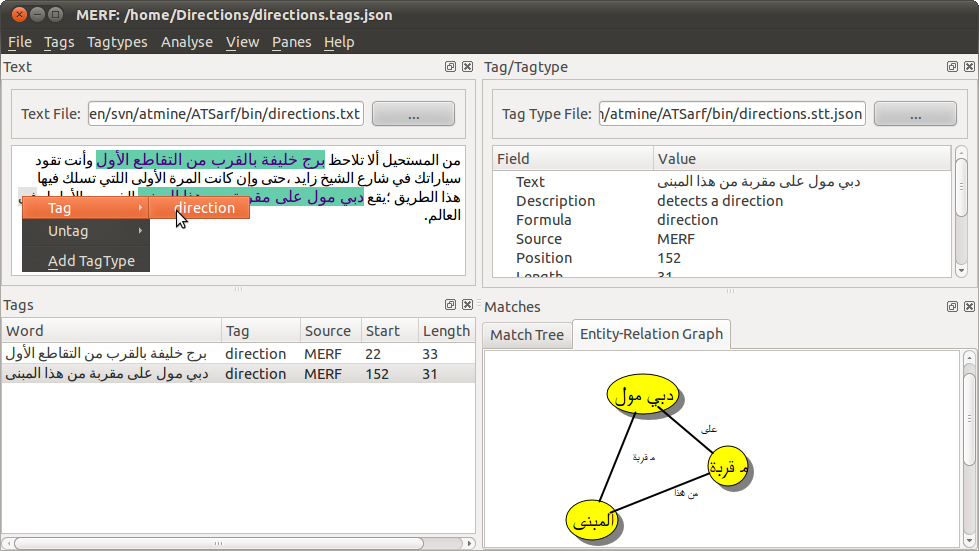
\includegraphics[width=0.9\textwidth]{figures/tagger}
  \caption{\framework main window with annotated text, tag descriptions, tag type legend properties, and manual tag edition menus. }
  \label{f:tagger}
\end{figure*}

\subsection{MBF Evaluation}
For each word $t_i \in T$, \framework computes a Boolean value 
($\{\mathit{true}, \mathit{false}\}$)
for all atomic terms. 
Then \framework computes Boolean values for all Boolean formulae. 
Then \framework computes the set of tags 
$R_i\subseteq T \times {\cal T}$  such that 
$(t_i,\mathit{tt}_j) \in R_i$ if and only if the Boolean formula $F_j$ associated with
tag type $\mathit{tt}_j$ is true for $t_i$. 

\subsection{MRE and Action Simulation}
For each MRE, 
\framework generates its equivalent non-deterministic finite automaton (NFA)~\cite{sipser2006introduction}. 
Each MRE operation has its equivalent representation in an NFA. 
As for the upto operation ($f$\textasciicircum$x$), 
it is equivalent to $f?|ff|\dots|\underbrace{f}_{n \text{ times}}$ which has an NFA mapping. 

Based on MBF evaluation stage, each word $t_i \in T$ is tagged by a tag set $R_i$. 
\framework simulates an NFA over the tag sets $R_i$ starting with $i=0,\dots,n$. 
A simulation match $m$ is a vector of the form $\langle r_i,r_{i+1},\dots,r_j\rangle$ where $0\le i\le j\le n~\text{and}~r_i\in R_i$. 
This tag match is equivalent to the text sequence match $\angle t_i,t_{i+1},\dots,t_j\rangle$ where $t_i\in T$. 

If the simulation has a match $\langle r_m,r_{m+1},\dots,r_n\rangle$ where $0\le m\le n\le n$, 
the next simulation starts at $R_{n+1}$. 
In case the NFA simulation has no match, the next simulation starts at $R_{m+1}$. 
If we have more than one match starting at $R_k$ where $0\le k\le n$, 
\framework returns the longest one.

\framework maintains a function $\phi\subset Q\times\Phi$, 
where $\mathit{Q}$ is the set of states in the NFA and $\Phi$ is the set of MREs in a formula. 
So $(q_i,f_j)\in\phi$ if state $q_i\in Q$ is generated by \framework in equivalence to $f_j\in\Phi$. 
\framework uses $\phi$ to retrieve the match tree with respect to the MRE formula. 
It also uses the map to execute the pre-match and on-match computational actions of an MRE based on current match.

\section{\framework GUI}
\label{sec:gui}
\framework~provides a user friendly interface to specify the 
atomic terms, the MBFs, the MREs, 
the tag types, and the legends. 
The GUI also allows the user to modify and correct the 
tag set $R$. 
The GUI allows the user also to compute accuracy results 
that compare different tag sets and that can serve well as 
inter annotation agreement results
when the tag sets come from two human annotators, 
or as evaluation results when comparing with reference tag sets.


%\framework saves the tags and the tag types in a user friendly format using
%the JavaScript Object Notation (JSON) format~\cite{nolan2014javascript}.
%The tag file keeps the paths of the separate text and tag type files. 
%It also contains a list of tags with their tag type identifiers,
%position in text, length, and word index.
%The tag type file contains MBF and MRE tag types. 
%%Each object has an array value containing the user-defined tag types. 
%Each tag type contains the name, description, expression, and the visualization legends.

%Figure~\ref{fig:mbftagger} shows the \framework GUI. 
%%\framework's GUI allows the user to create, manipulate, and analyze a project. 
%The {\em File} menu is used to create, close, or open an existing project. 
%The {\em Tags} menu enables the user to manually define and edit tag types. 
%The user can define and edit the MBF and MRE based tag types and 
%start the corresponding automatic morphology-based simulators from the {\em Tagtypes} menu. 
%The user performs comparison and analysis of two tag sets using the {\em Analyse} menu. 
%{\em View} menu enables the user to switch visualization modes of the tags. 

\subsection{Tag type Boolean formula editor}
The user writes MBF tag types with the tag type editor introduced in~\cite{JaZaMatar}. %shown in Figure~\ref{f:bfe}.
First the user specifies atomic terms by selecting a feature from ${\cal F}$. 
%The pattern filters the feature values.
The user can also choose whether to require an exact match using the
\cci{isA} predicate, or a substring match using the
\cci{contains} predicate option.

The user can add and remove feature values to the atomic terms 
using push buttons. 
A check box in the ``Feature'' column allows negating the term, and the
``Relation'' column switches the predicate between 
\cci{isA} and \cci{contains}. 
The list of feature and value pairs is interpreted as a disjunction to form
the MBF. 
A right pane shows a description of the tag type and a set of legend 
descriptors. 
When the stem or gloss features are selected, the user has the option to 
use the $Syn^k$ feature. 
%The user selects the check box in the lower left of the editor and sets the order in the spin box.

In the direction extraction task example, the user specifies four MBF-based 
tag types with labels 
$N$, $P$, $R$, and $U$ with  ``name of person'', ``name of place'', 
``relative position'', and ``numerical term'' descriptions, respectively. 
For each MBF, the user selects the morphological features, 
specifies the constant value $CF$, and adds it to the Boolean formula editor. 
%The user also assigns legend descriptors to each defined tag type. 
%
%Figure~\ref{f:bfe} shows the $U$ MBF which requires the gloss tag of 
%the stem to be an exact match of either {\tt first}, {\tt second}, \dots, or {\tt tenth}. 
%The legend descriptors set foreground and background colors to {\tt orangered}, 
%and {\tt gray}, respectively, and the font size to {\tt 12}.
%, normal font weight, and unitalicized.

\subsection{MBF match visualization}

%After defining the MBFs of the direction extraction task, 
%the user calls the MBF simulator from the {\tt Tagtypes} menu. 
%The snapshot in Figure~\ref{fig:mbftagger} shows 
The MBF match visualizer shows color sensitive text view, the tag list view, and the tag description view. 
%The color-sensitive text view shows the text with visualization of the MBF tag type matches. 
%The tag list view shows all tags.
%that are automatically or manually applied to the text. 
The tag description view presents the details of the selected tag along with 
the relevant tag type information.
%
The user can edit the tags using a context sensitive menus. 
\framework GUI also allows manual tag types and corresponding tags 
that are not based on morphological features.
This enables building reference corpora without 
help from the morphological analyzer.

\begin{figure}[tb]
  \centering
  {\setlength{\fboxsep}{0pt}%
  \setlength{\fboxrule}{0.5pt}%
  \fbox{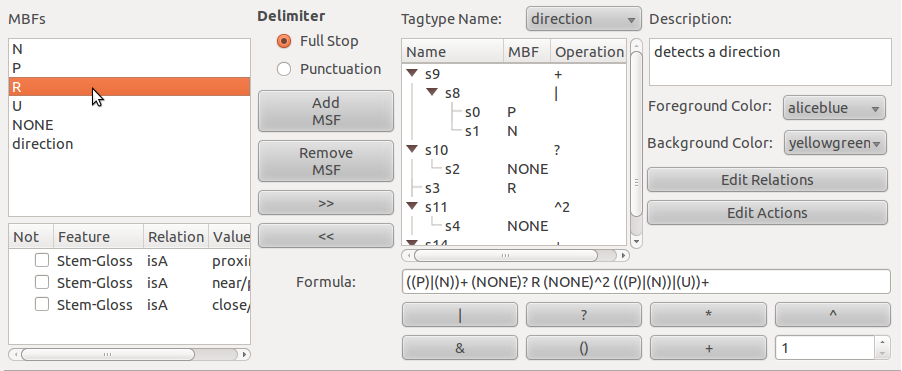
\includegraphics[width=0.995\textwidth]{figures/mreedit}}}
  \vspace{-2em}
  \caption{\label{f:sfe}\framework tag type regular expression editor.}
\end{figure}

\subsection{Tag type regular expression editor}
\vspace{-1em}

After interacting with the MBF editor, the user moves to 
specify the regular expressions. 
The MRE editor of Figure~\ref{f:sfe} allows the 
definition of an MRE tag type in a user friendly manner. 
The user first adds the required MBF formulae 
by selecting a label from ${\cal T}$ under MBFs. 
The Boolean formula of a highlighted tag type is shown in the table on the lower left pane. 
Each selected MBF is associated with an automatic name. 
The user can nest the MRE expression using a tree view of the MRE operations. 
The tree features the name, MBF, and operation for each sub-expression. 
%Moreover, a defined MRE is directly added to the MBF list enabling substitution and recursion 
%in formula definition.

%{\tt NONE} is a special tag type with no Boolean formula. 
%It tags all the words that are not tagged with any of the morphology-based Boolean tag types. 
%{\tt NONE} is defined by default and can be used to introduce flexibility and noise tolerance into the formula. 
%We previously defined this tag type in Section~\ref{sec:framework} and referred to it by $O$ (other).

%The regular expression editor enables the user to apply operations to the selected expressions. 
To specify a binary operation the user selects two sub-expressions and clicks the corresponding
operation button. 
%To do so, the user selects one or two expressions then selects an operation from the ones shown 
%in the lower left of the view. 
The operations include disjunction, conjunction, zero or one, sequence, zero or more, 
one or more, and up to a user defined constant.
The right pane shows a description of the tag type and a set of legend 
descriptors. 

%\[
%	(P|N)+~\mathit{O}?~R~\mathit{O^{\wedge}2}~(P|N|U)+
%\]
%In the direction task, we aim to build the expression shown above. 
%Thus we start by adding the MBFs $P$, $N$, $\textit{NONE}$, $R$, $\textit{NONE}$, $P$, $N$, and $U$. 
%We apply the required operations incrementally to build the final expression. 
%For example, we apply the disjunction ($|$) operation to the first $P$ and $N$ added, 
%then we apply the one or more ($+$) operation to the resulting sub-expression.
%We proceed as such to build the regular expression shown in Figure~\ref{f:sfe}. 
%Similar to the MBF tag type editor, the user specifies a set of legend descriptors for each MRE tag type.
%

\vspace{-1em}
\subsection{MRE match visualization}

While specifying an MRE the user can interact with the visualization and editor views
to make sure the MRE expresses the intent. 
The color-sensitive text view in Figure~\ref{fig:treegraph} shows 
the highlighted tag matches after the user called the MRE simulator using 
the {\tt Tagtypes} menu. 

The \major{matching parse tree} view shows the selected match in a graph view.
Figure~\ref{fig:treegraph} shows the \major{matching parse tree} of the direction task 
\RL{dby mwl `l_A mqrbT mn h_dA Almbn_A}(Dubai Mall is located near this building). 
%Leaf nodes show the match text, internal nodes show the operations, and edge labels shows the MBF tag type name.

\begin{figure}[tb]
  \centering
  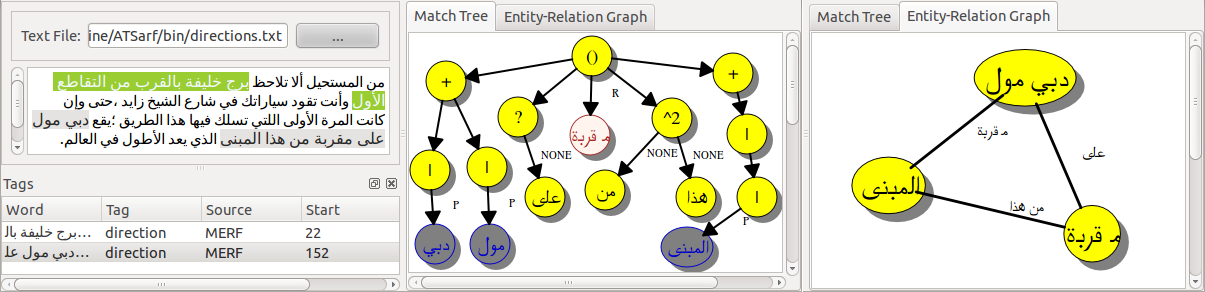
\includegraphics[width=\textwidth]{figures/treegraph}
  \vspace{-2em}
  \caption{\label{fig:treegraph}MRE annotated Text, MRE \major{matching parse tree}, and entity-relation graph.}
\end{figure}

%\begin{figure}[tb]
%  \centering
%  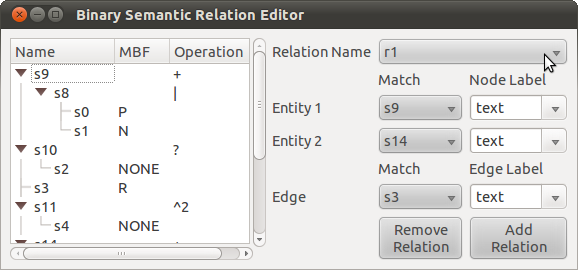
\includegraphics[width=0.5\textwidth]{figures/merfsreditor.png}
%\caption{\framework~relation editor}
%  \label{fig:relationeditor}
%\end{figure}

\subsection{User defined relation editor}

After the user is satisfied with the MRE matches, 
the user moves to define relations and code actions. 
The relation editor allows the user to define relations 
by specifying $\langle e_1,e_2,r\rangle$ tuples, 
where $e_1$ and $e_2$ denote source and destination entities, and $r$ denotes 
the label.
The editor shows the MRE tree and allows the user to select the sub 
expressions and select features 
of the matches of the sub expressions to define the three components of the relation. 

A snapshot of the GUI in 
Figure~\ref{fig:treegraph} shows in an interactive graph view
the entity-relation graph of the match of the user defined relation 
extracted from the \major{matching parse tree} of the MRE. 
%
In the computational action editor, an advanced user can 
enter C++ code and use the \framework API to program and process 
subexpression matches. 
%RE matches In order to add computational actions to an MRE sub-expression, 
%the user selects to edit the actions in the MRE tag type editor. 
%The view allows the user to specify the actions in a user friendly manner. 
%\framework provides the user with an API to access the sub-expression match features easily and define the pre-match actions. 
%The match features include the text, position, length, and numerical value if applicable, and morphological features for MBF matches. 
%\framework also enables the user to add C++ declarations and library includes.

\subsection{Analysis}

In the analysis view, the user provides 
two tag sets $R_1$ and $R_2$ and 
two tag type sets ${\cal T}_1$ and ${\cal T}_2$ as input. 
%The analysis view provides views of the differences between the tag types and 
%the tag sets.
%
The tag type difference view shows the text annotated in three panes: 
(i) the common tag types ${\cal T}_1 \cap {\cal T}_2$,
(ii) the tag types in ${\cal T}_1$ but not in ${\cal T}_2$, 
and (iii) the tag types in ${\cal T}_2$ and not in ${\cal T}_1$.
%
Similarly, the tag difference view shows $R_1\cap R_2$, $R_1/R_2$ and $R_2/R_1$
in addition to precision, recall and F-measure values. 
The user selects a predicate to compute the metrics from the following predicates:
(1) ``Intersection'': a tag from $R_1$ intersects in text with a tag in $R_2$,
(2) ``Exact'': a tag from $R_1$ exactly matches a tag in $R_2$,
(3) ``A includes B'': a tag from $R_1$ contains a tag from $R_2$, and
(4) ``B includes A'': a tag from $R_2$ contains a tag from $R_1$.


\section{Implementation}
\label{sec:implementation}
In this Section, we describe the different implementation aspects of \framework. 
We cover the data model used to store the MBF and MRE based tag types, the MBF and MRE tags, and the generated actions. 
We explain the data structures used to hold the data from the files including MBF and MRE tag types, MBF and MRE matches, code action, and relations. 
Then, we describe the simulation of the MBFs and MREs to compute the matches, the construction of relations matches, and the execution of actions. 
We also describe how the interface is written with Qt and how the match tree and entity-relation graphs are visualized.

\subsection{Data Model}

\framework saves the tag types and the tags in a user friendly format using
the JavaScript Object Notation (JSON) data-interchange format~\cite{nolan2014javascript}.
The JSON interface is built on two structures.
The first structure is a collection of name and value pairs. An instance
of the structure is referred to as an object. 
The second structure defines ordered lists of values as arrays. 
The name in a name value pair is an identifier string 
and the value can be a string, a number, a Boolean (true or false), an object, 
or an array. 
%The file format is selected to make it easier to compute statistical metrics 
%necessary for CL and NLP tasks such as frequency and distance.

\subsubsection{Tag file}

The tag file keeps the paths of the separate text and tag type files. 
It also contains a list of tags with their tag type identifiers as well 
as their position in text in terms of number of characters from the beginning 
of text, length of the tag, and word index. 
In addition to the previous features, 
the MRE matches contain an object representing the match tree with 
the identifier ``match''.

\begin{figure}[h*]
\begingroup
    \fontsize{8pt}{12pt}\selectfont
\begin{verbatim}
{ "TagArray":
  [{"length": 3,"pos": 152,"source": 1,"type": "P","wordIndex": 29},...],
  "simulationTags":
  [{"formula": "direction","length": 33,"match": {...},"pos": 22,"source": 1},...],
  "TagTypeFile":"directions.stt.json",
  "file":"directions.txt",
  "textchecksum":211
}
\end{verbatim}
\endgroup
\caption{Tag file format}
\label{fig:tagfile}
\end{figure}

A sample tag file is shown in Figure~\ref{fig:tagfile}. 
The tag file includes the tag type file pointer(TagTypeFile), 
text file pointer (file), the list of MBF tags (TagArray), 
the list of MRE tags (simulationTags), 
and {\em textchecksum} which is used to ensure that the 
text is not corrupt. 
An MBF tag is defined by its position in the text (pos), length of the tag (length), 
tag type (type), word index (wordIndex), and the source of the tag (source). 
A simulation tag, referring to an MRE match, is defined by the formula (MRE), length, position and the match tree (match).

\subsubsection{Tag type file}

The tag type file contains two objects referring to MBF and MRE based tag types. 
Each object has an array value containing the user-defined tag types. 
Each tag type is stored as an object and contains the name, description, formula or expression, and the visualization legends.

\begin{figure}[h!]
\begingroup
    \fontsize{8pt}{12pt}\selectfont
\begin{multicols}{2}
\begin{verbatim}
{ "TagTypeSet":
  [{"Description":"numerical term",
   "Features":[{"Negation": "",
                "Relation": "isA",
                "Stem-Gloss": "first"},
                ... 
              ],
   "Tag": "U",
   "background_color": "grey",
   "bold": false,
   "font": 12,
   "foreground_color": "orangered",
   "italic": false,
   "underline": false
   },...
  ],

  
  "MSFs": [{
      "name": "direction","description": "",
  	  "MSF": {... {"MBF": "U","actions": "",
  	               "init": "","name": "s7",
  	               "parent": "s13","type": "mbf"} 
  	               ... 
  	         },
  	  "Relations": [...
  	           { "entity1": "s9","e1Label": "text",
  	             "entity2": "s14","e2Label": "text",
  	             "edge": "s3","edgeLabel": "text",
  	             "name": "r1"} 
  	             ... ],
      "bgcolor": "#9acd32","fgcolor": "#f0f8ff",
      "includes": "","members": "",
      "delimiter": true
     }]
}
\end{verbatim}
\end{multicols}
\endgroup
\caption{Tag type file format}
\label{fig:tagtypefile}
\end{figure}

Figure~\ref{fig:tagtypefile} shows a sample tag type file. 
The file includes a list of defined MBF tag types (TagTypeSet). 
Each tag type is defined by the fields name (Tag), description, 
morphological features (Features), foreground color, 
background color, bold, italic, underline, font size (font), and id. 
The morphological features are stored in an array of objects where each object refers to an MAT. 
An MAT object contains the fields negation, relation (isA or contains), and feature name and value pair.

The file also includes a list of defined MRE tag types and refers to them with the
notation Morphology-based Sequential Formulae (MSFs); the tool name of MRE. 
Each tag type is defined by the fields name, description, expression, 
semantic relations (Relations), code action information (includes and members), 
delimiter, and foreground and background color. 
The includes and members contain the libraries and global variables added to the actions by the user respectively. 

The expression is a tree of objects and arrays whose depends on the definition of the user. 
For example, a sequence of sub-expressions is expressed as an array of objects. 
A sample MBF added to the expression is shown in the Figure	defined by the name (MBF), pre-match actions (init), on-match actions (actions), unique name assigned by \framework(name), name of parent expression (parent), and expression type (type) which is specified based on operation applied. 
The delimiter entry specifies whether the simulation should stop on a full stop or any punctuation mark.

Relations are saved in an array where each relation is defined by its name, the first entity (entity1) and its label (e1Label), second entity (entity2) and its label (e2Label), and the edge and its label (edgeLabel).


The user-defined actions (pre-match and on-match) are written into a cpp output file. 
The file includes the libraries included, global members declared, pre-match and on-match functions, and the function calls. 
A sample of the generated file is shown in Figure~\ref{fig:generatedactions}. 
The Figure shows a sample on-match function for a sub-expression named {\tt s2} (s2\_Match). 
The function takes an integer as a parameter. 
The integer refers to the numerical value of the match of {\tt s2} (s2\_number). 
The second function named {\tt number\_actions} contains the list of function calls. 
A sample call of the s2\_Match is shown with the parameter value 200.

\begin{figure}[h!]
%\begingroup
%    \fontsize{8pt}{12pt}\selectfont
\begin{multicols}{2}
\begin{Verbatim}[fontsize=\relsize{-2}] 
extern "C" void s2_onMatch(int s2_number) {
   isHundred = true;
   if(current == 0)  {
      currentH=s2_number;
   }
   else {
      if(!isKey) {
         currentH= current * s2_number;
         current = 0;
      }
      else {
         currentH = s2_number;
      }
   }
   isKey = false;
}
extern "C" void number_actions() {
   s5_preMatch();
   s4_preMatch();
   s2_preMatch();
   s2_onMatch(200);
   s4_onMatch();
   s4_preMatch();
   s3_preMatch();
   s0_preMatch();
   s0_onMatch(9);
   .
   .
   .
}


\end{Verbatim}
\end{multicols}
%\endgroup
\caption{sample generated actions file}
\label{fig:generatedactions}
\end{figure}

\subsection{Data structures}

In this section, we explain the data structures we used to store the text, MBF-based tag types, 
MRE-based tag types, relations, MBF matches, MRE match trees, and relations constructed.

\subsubsection{Arabic document}

\framework supports Arabic documents with UTF-8 encoding only. 
The input Arabic text is saved as a string. 
We process the text to build a word position to word index hash, 
a set of words that end by punctuation, and a set of words that end with full stop. 
The two sets are used in MRE simulation.

\subsubsection{MBF tag types}

We store the MBF tag types in a vector of {\tt TagType} class. 
Each tag type contains strings to store the name, description, foreground color, and background color. 
Boolean variables are used to track the bold and italic properties. 
The Boolean formula is stored as a vector of quadruples where each quadruple contains the feature, feature value, negation option, and predicate (isA or contains).

\subsubsection{MRE tag types}

The MRE tag types are stored in a vector of {\tt MSFormula} class. 
The regular expression is stored in a tree structure where each node refers to a sub-expression. 
Each sub-expression is represented by a class derived from a base class called {\tt MSF}. 
{\tt MSF} defines the common attributes of all sub-expressions including name, pre-match code actions, and on-match code actions. 
It also contains the common functions required to be implemented by all derived classes.

An MRE tag type is stored in a class called MSFormula. 
This class contains strings for description of the tag type, foreground color, 
background color, included libraries by user, and action global variables. 
It also contains a vector of MSF pointers referring to a sequence of sub-expressions. 
MSFormula contains a formula that maps the name of each sub-expression to a pointer of the relevant structure instance.

The expressions with the operations zero or one ($?$), 
zero or more ($*$), one or more ($+$), and zero up to x ($f$\textasciicircum$x$) 
are stored in a class called {\tt UNARYF}. 
This class holds the operation and an MSF pointer referring to the sub-expression subject to the operation. 
The expressions with the disjnuction ($|$) or conjunction ($\&$) operations 
are stored in a class called {\tt BINARYF}. 
This class holds the operation along with two MSF pointers referring to the two sub-expressions subject to conjunction or disjunction. 
The sequential expression is stored in a class called {\tt SequentialF}. 
It contains a vector of MSF pointers referring to a sequence of sub-expressions. 
An MBF-based sub-expression is stored in a class called {\tt MBF} which contains the name of the MBF tag type. 
All the classes introduced above are derived from the base class {\tt MSF}.

Moreover, the MRE tag type stores the relevant semantic relations defined by the user. 
The relations are stored in a vector and each relation is represented by a class {\tt Relation}. 
This class holds MSF pointers that refer to the three entity sub-expressions, and strings to identify the name of the relation and the labels of the three entities.

\subsubsection{MBF tags}

The MBF tags are stored in a multi-hash based on wordindex. 
We use a multi-hash because a single word can have multiple tags as stated before. 
Each tag is represented in an instance of the {\tt Tag} class. 
This class holds a pointer to the tag type, and integers for word index, position, and length. 
It also contains a flag to differentiate the automatic tag from a user one.

\subsubsection{MRE tags}
\label{subsubsec:mretag}

We store the MRE tag type matches in a vector of {\tt Match} class. 
In order to preserve the relation between the expression and the match tags, we use similar classes to store the match in a tree structure as well. 
Hence, we define the classes {\tt KeyM}, {\tt UnaryM}, {\tt BinaryM}, and {\tt SequentialM} referring to MBF, UNARYF, BINARYF, and SequentialF matches, respectively. 
All those classes inherit from base class {\tt Match}.

The base class contains common data including pointer to relevant MSF, 
operation if present, and a flag to differentiate the automatic tag from a user one. 
KeyM holds the matching word, tag name (key), position, and length. 
UnaryM contains a vector of {\tt Match} pointers and an integer to the limit in UPTO operation if applicable. 
BinaryM contains two {\tt Match} pointers. 
Both pointers are required in the conjunction case, but only one is used in the disjunction. 
The SequentialM class holds a vector of {\tt Match} pointers.

\subsection{MBF simulation}

The Arabic morphological analyzer, Sarf, provides a pure virtual function called $on\_match$. 
This function is triggered by the analyzer for every morphological solution computed for an input word. 
Through this function, we can access the morphological features of the solution including the stem, affixs, POS and gloss tags, and categories.

We derive the class {\tt SarfTag} from {\tt Stemmer}, the main class of Sarf, and implement the $on\_match$ function. 
For each solution found, we iterate over the MBFs and check whether the solution matches any of the MATs defined by the user. 
In case there is a match, we add a tag to the multi-hash referring to the word index. 
The tag contains a pointer to the tag type that refers to the matching MBF. 

In order to minimize the computational cost of the $Syn^k$ feature, we compute the sets prior to the tag computation process. 
For each $CS$ (constant stem) and $k$ (order) pair, we compute the set of Arabic stems that are synonyms of the stem $CS$ of order $k$. 
When we find a $Syn^k$ based MAT in the tag computation process, we detect a match if a solution stem belongs to the relevant set.

\subsection{MRE simulation}

In this Section, we describe how we generate the NFA equivalent to the MRE. 
Then we describe how we simulate the NFA and construct the match trees.

\subsubsection{NFA generation}

In order to simulate the regular expression, we first generate the equivalent non-deterministic finite automata (NFA). 
We represent the generated NFA with the {\tt NFA} class which contains strings representing start and accept states, a multi-map for transitions, and a map from NFA state to relevant MSF. 
The state name is represented by a string of the form $q_0$, $q_1$, \dots
The transition multi-hash takes a concatenation of current state and label (epsilon or tag type name). 
It the transition exists, the hash returns one or more transition states. 
A sample transition input is $q_1|NONE$ and a sample value would be $q_2$ if the transition exists. 
The MSF map is used to track the source sub-expression of each state and whether the state was generated with a pre-match or on-match property. 
This information is important in the simulation of the NFA, and computation of the match tree. 
Thus, the map takes the state name as input and returns a pair of MSF pointer and string indicating the pre-match or on-match property.

\begin{figure}[h!]
\centering
\resizebox{0.7\columnwidth}{!}{
	\relsize{-3} % Graphic for TeX using PGF
% Title: /home/ameen/Desktop/starNFA.dia
% Creator: Dia v0.97.1
% CreationDate: Tue Jan 14 10:32:26 2014
% For: ameen
% \usepackage{tikz}
% The following commands are not supported in PSTricks at present
% We define them conditionally, so when they are implemented,
% this pgf file will use them.
\ifx\du\undefined
  \newlength{\du}
\fi
\setlength{\du}{15\unitlength}
\begin{tikzpicture}
\pgftransformxscale{1.000000}
\pgftransformyscale{-1.000000}
\definecolor{dialinecolor}{rgb}{0.000000, 0.000000, 0.000000}
\pgfsetstrokecolor{dialinecolor}
\definecolor{dialinecolor}{rgb}{1.000000, 1.000000, 1.000000}
\pgfsetfillcolor{dialinecolor}
\definecolor{dialinecolor}{rgb}{1.000000, 1.000000, 1.000000}
\pgfsetfillcolor{dialinecolor}
\fill (21.568700\du,12.550000\du)--(21.568700\du,14.975000\du)--(27.468700\du,14.975000\du)--(27.468700\du,12.550000\du)--cycle;
\definecolor{dialinecolor}{rgb}{1.000000, 1.000000, 1.000000}
\pgfsetfillcolor{dialinecolor}
\pgfpathmoveto{\pgfpoint{21.568713\du}{12.550000\du}}
\pgfpatharc{270}{180}{0.500000\du and 0.500000\du}
\pgfusepath{fill}
\definecolor{dialinecolor}{rgb}{1.000000, 1.000000, 1.000000}
\pgfsetfillcolor{dialinecolor}
\pgfpathmoveto{\pgfpoint{27.968700\du}{13.050000\du}}
\pgfpatharc{360}{270}{0.500000\du and 0.500000\du}
\pgfusepath{fill}
\definecolor{dialinecolor}{rgb}{1.000000, 1.000000, 1.000000}
\pgfsetfillcolor{dialinecolor}
\fill (21.068700\du,13.050000\du)--(21.068700\du,14.475000\du)--(27.968700\du,14.475000\du)--(27.968700\du,13.050000\du)--cycle;
\definecolor{dialinecolor}{rgb}{1.000000, 1.000000, 1.000000}
\pgfsetfillcolor{dialinecolor}
\pgfpathmoveto{\pgfpoint{21.068700\du}{14.474974\du}}
\pgfpatharc{180}{90}{0.500000\du and 0.500000\du}
\pgfusepath{fill}
\definecolor{dialinecolor}{rgb}{1.000000, 1.000000, 1.000000}
\pgfsetfillcolor{dialinecolor}
\pgfpathmoveto{\pgfpoint{27.468661\du}{14.975000\du}}
\pgfpatharc{90}{0}{0.500000\du and 0.500000\du}
\pgfusepath{fill}
\pgfsetlinewidth{0.020000\du}
\pgfsetdash{{1.000000\du}{0.200000\du}{0.200000\du}{0.200000\du}{0.200000\du}{0.200000\du}}{0cm}
\pgfsetdash{{1.000000\du}{0.200000\du}{0.200000\du}{0.200000\du}{0.200000\du}{0.200000\du}}{0cm}
\pgfsetmiterjoin
\definecolor{dialinecolor}{rgb}{0.000000, 0.000000, 0.000000}
\pgfsetstrokecolor{dialinecolor}
\draw (21.568700\du,12.550000\du)--(27.468700\du,12.550000\du);
\definecolor{dialinecolor}{rgb}{0.000000, 0.000000, 0.000000}
\pgfsetstrokecolor{dialinecolor}
\draw (21.568700\du,14.975000\du)--(27.468700\du,14.975000\du);
\definecolor{dialinecolor}{rgb}{0.000000, 0.000000, 0.000000}
\pgfsetstrokecolor{dialinecolor}
\pgfpathmoveto{\pgfpoint{21.568713\du}{12.550000\du}}
\pgfpatharc{270}{180}{0.500000\du and 0.500000\du}
\pgfusepath{stroke}
\definecolor{dialinecolor}{rgb}{0.000000, 0.000000, 0.000000}
\pgfsetstrokecolor{dialinecolor}
\pgfpathmoveto{\pgfpoint{27.968700\du}{13.050000\du}}
\pgfpatharc{360}{270}{0.500000\du and 0.500000\du}
\pgfusepath{stroke}
\definecolor{dialinecolor}{rgb}{0.000000, 0.000000, 0.000000}
\pgfsetstrokecolor{dialinecolor}
\draw (21.068700\du,13.050000\du)--(21.068700\du,14.475000\du);
\definecolor{dialinecolor}{rgb}{0.000000, 0.000000, 0.000000}
\pgfsetstrokecolor{dialinecolor}
\draw (27.968700\du,13.050000\du)--(27.968700\du,14.475000\du);
\definecolor{dialinecolor}{rgb}{0.000000, 0.000000, 0.000000}
\pgfsetstrokecolor{dialinecolor}
\pgfpathmoveto{\pgfpoint{21.068700\du}{14.474974\du}}
\pgfpatharc{180}{90}{0.500000\du and 0.500000\du}
\pgfusepath{stroke}
\definecolor{dialinecolor}{rgb}{0.000000, 0.000000, 0.000000}
\pgfsetstrokecolor{dialinecolor}
\pgfpathmoveto{\pgfpoint{27.468661\du}{14.975000\du}}
\pgfpatharc{90}{0}{0.500000\du and 0.500000\du}
\pgfusepath{stroke}
% setfont left to latex
\definecolor{dialinecolor}{rgb}{0.000000, 0.000000, 0.000000}
\pgfsetstrokecolor{dialinecolor}
\node at (24.518700\du,13.865833\du){};
\definecolor{dialinecolor}{rgb}{1.000000, 1.000000, 1.000000}
\pgfsetfillcolor{dialinecolor}
\pgfpathellipse{\pgfpoint{19.746200\du}{13.736482\du}}{\pgfpoint{0.697500\du}{0\du}}{\pgfpoint{0\du}{0.586482\du}}
\pgfusepath{fill}
\pgfsetlinewidth{0.020000\du}
\pgfsetdash{}{0pt}
\pgfsetdash{}{0pt}
\pgfsetmiterjoin
\definecolor{dialinecolor}{rgb}{0.000000, 0.000000, 0.000000}
\pgfsetstrokecolor{dialinecolor}
\pgfpathellipse{\pgfpoint{19.746200\du}{13.736482\du}}{\pgfpoint{0.697500\du}{0\du}}{\pgfpoint{0\du}{0.586482\du}}
\pgfusepath{stroke}
% setfont left to latex
\definecolor{dialinecolor}{rgb}{0.000000, 0.000000, 0.000000}
\pgfsetstrokecolor{dialinecolor}
\node at (19.746200\du,13.839815\du){$q_i$};
\definecolor{dialinecolor}{rgb}{1.000000, 1.000000, 1.000000}
\pgfsetfillcolor{dialinecolor}
\pgfpathellipse{\pgfpoint{29.328700\du}{13.721482\du}}{\pgfpoint{0.697500\du}{0\du}}{\pgfpoint{0\du}{0.586482\du}}
\pgfusepath{fill}
\pgfsetlinewidth{0.020000\du}
\pgfsetdash{}{0pt}
\pgfsetdash{}{0pt}
\pgfsetmiterjoin
\definecolor{dialinecolor}{rgb}{0.000000, 0.000000, 0.000000}
\pgfsetstrokecolor{dialinecolor}
\pgfpathellipse{\pgfpoint{29.328700\du}{13.721482\du}}{\pgfpoint{0.697500\du}{0\du}}{\pgfpoint{0\du}{0.586482\du}}
\pgfusepath{stroke}
% setfont left to latex
\definecolor{dialinecolor}{rgb}{0.000000, 0.000000, 0.000000}
\pgfsetstrokecolor{dialinecolor}
\node at (29.328700\du,13.824815\du){$q_j$};
\definecolor{dialinecolor}{rgb}{1.000000, 1.000000, 1.000000}
\pgfsetfillcolor{dialinecolor}
\pgfpathellipse{\pgfpoint{22.156200\du}{13.721482\du}}{\pgfpoint{0.697500\du}{0\du}}{\pgfpoint{0\du}{0.586482\du}}
\pgfusepath{fill}
\pgfsetlinewidth{0.020000\du}
\pgfsetdash{}{0pt}
\pgfsetdash{}{0pt}
\pgfsetmiterjoin
\definecolor{dialinecolor}{rgb}{0.000000, 0.000000, 0.000000}
\pgfsetstrokecolor{dialinecolor}
\pgfpathellipse{\pgfpoint{22.156200\du}{13.721482\du}}{\pgfpoint{0.697500\du}{0\du}}{\pgfpoint{0\du}{0.586482\du}}
\pgfusepath{stroke}
% setfont left to latex
\definecolor{dialinecolor}{rgb}{0.000000, 0.000000, 0.000000}
\pgfsetstrokecolor{dialinecolor}
\node at (22.156200\du,13.824815\du){$q_m$};
\definecolor{dialinecolor}{rgb}{1.000000, 1.000000, 1.000000}
\pgfsetfillcolor{dialinecolor}
\pgfpathellipse{\pgfpoint{26.808700\du}{13.721482\du}}{\pgfpoint{0.697500\du}{0\du}}{\pgfpoint{0\du}{0.586482\du}}
\pgfusepath{fill}
\pgfsetlinewidth{0.020000\du}
\pgfsetdash{}{0pt}
\pgfsetdash{}{0pt}
\pgfsetmiterjoin
\definecolor{dialinecolor}{rgb}{0.000000, 0.000000, 0.000000}
\pgfsetstrokecolor{dialinecolor}
\pgfpathellipse{\pgfpoint{26.808700\du}{13.721482\du}}{\pgfpoint{0.697500\du}{0\du}}{\pgfpoint{0\du}{0.586482\du}}
\pgfusepath{stroke}
% setfont left to latex
\definecolor{dialinecolor}{rgb}{0.000000, 0.000000, 0.000000}
\pgfsetstrokecolor{dialinecolor}
\node at (26.808700\du,13.824815\du){$q_n$};
\pgfsetlinewidth{0.020000\du}
\pgfsetdash{}{0pt}
\pgfsetdash{}{0pt}
\pgfsetbuttcap
{
\definecolor{dialinecolor}{rgb}{0.000000, 0.000000, 0.000000}
\pgfsetfillcolor{dialinecolor}
% was here!!!
\pgfsetarrowsend{latex}
\definecolor{dialinecolor}{rgb}{0.000000, 0.000000, 0.000000}
\pgfsetstrokecolor{dialinecolor}
\pgfpathmoveto{\pgfpoint{26.315542\du}{13.306807\du}}
\pgfpatharc{303}{238}{3.425154\du and 3.425154\du}
\pgfusepath{stroke}
}
\pgfsetlinewidth{0.020000\du}
\pgfsetdash{}{0pt}
\pgfsetdash{}{0pt}
\pgfsetbuttcap
{
\definecolor{dialinecolor}{rgb}{0.000000, 0.000000, 0.000000}
\pgfsetfillcolor{dialinecolor}
% was here!!!
\pgfsetarrowsend{latex}
\definecolor{dialinecolor}{rgb}{0.000000, 0.000000, 0.000000}
\pgfsetstrokecolor{dialinecolor}
\pgfpathmoveto{\pgfpoint{19.745587\du}{14.322626\du}}
\pgfpatharc{119}{62}{9.914679\du and 9.914679\du}
\pgfusepath{stroke}
}
\pgfsetlinewidth{0.020000\du}
\pgfsetdash{}{0pt}
\pgfsetdash{}{0pt}
\pgfsetbuttcap
{
\definecolor{dialinecolor}{rgb}{0.000000, 0.000000, 0.000000}
\pgfsetfillcolor{dialinecolor}
% was here!!!
\pgfsetarrowsend{latex}
\definecolor{dialinecolor}{rgb}{0.000000, 0.000000, 0.000000}
\pgfsetstrokecolor{dialinecolor}
\draw (27.506200\du,13.721482\du)--(28.631200\du,13.721482\du);
}
\pgfsetlinewidth{0.020000\du}
\pgfsetdash{}{0pt}
\pgfsetdash{}{0pt}
\pgfsetbuttcap
{
\definecolor{dialinecolor}{rgb}{0.000000, 0.000000, 0.000000}
\pgfsetfillcolor{dialinecolor}
% was here!!!
\pgfsetarrowsend{latex}
\definecolor{dialinecolor}{rgb}{0.000000, 0.000000, 0.000000}
\pgfsetstrokecolor{dialinecolor}
\draw (20.443700\du,13.736482\du)--(21.458700\du,13.721482\du);
}
% setfont left to latex
\definecolor{dialinecolor}{rgb}{0.000000, 0.000000, 0.000000}
\pgfsetstrokecolor{dialinecolor}
\node[anchor=west] at (19.0\du,12.825000\du){$s_k|pre$};
% setfont left to latex
\definecolor{dialinecolor}{rgb}{0.000000, 0.000000, 0.000000}
\pgfsetstrokecolor{dialinecolor}
\node[anchor=west] at (28.50\du,12.900000\du){$s_k|on$};
% setfont left to latex
\definecolor{dialinecolor}{rgb}{0.000000, 0.000000, 0.000000}
\pgfsetstrokecolor{dialinecolor}
\node[anchor=west] at (20.6\du,13.525000\du){$\epsilon$};
% setfont left to latex
\definecolor{dialinecolor}{rgb}{0.000000, 0.000000, 0.000000}
\pgfsetstrokecolor{dialinecolor}
\node[anchor=west] at (27.9\du,13.490000\du){$\epsilon$};
% setfont left to latex
\definecolor{dialinecolor}{rgb}{0.000000, 0.000000, 0.000000}
\pgfsetstrokecolor{dialinecolor}
\node[anchor=west] at (24.426200\du,13.090000\du){$\epsilon$};
% setfont left to latex
\definecolor{dialinecolor}{rgb}{0.000000, 0.000000, 0.000000}
\pgfsetstrokecolor{dialinecolor}
\node[anchor=west] at (24.428700\du,15.315000\du){$\epsilon$};
\end{tikzpicture}

}
\caption{Star expression NFA}
\label{fig:starnfa}
\end{figure}

Figure~\ref{fig:starnfa} shows a sample NFA generated for a zero or more expression ($*$). 
The dotted block represents the sub-expression subject to the zero or more operation. 
$q_i$ is the start state of this expression and $q_j$ is the end state. 
The map entry of the start state is $s_k$ concatenated with $pre$. 
$s_k$ is the name of the stared expression and $pre$ refers to pre-match. 
Similarly, $on$ in the $q_j$ entry refers to on-match.

\subsubsection{NFA simulation}

We simulate the generated NFA in a recursive function. 
The function takes as parameters a pointer to the NFA, current state, and current word index and returns a {\tt Match} instance. 
At each stage, we check for possible transitions from current state based on empty strings ($\epsilon$) or MBF tags. 
Note that we can get the tags for current word index using the multi-hash used to store the MBF tag based on word index.

When we reach the accept state, we build the match tree backwards. 
At each stage, we check if the current state refers to a sub-expression pre-match or on-match property. 
On an on-match property, we generate the relevant match node compatible with the sub-expression type (Subsubsection~\ref{subsubsec:mretag}) and add it as a child node to returned {\tt Match} structure. 
In case of a pre-match property, we return the parent node of the {\tt Match} structure.

\subsection{Code action execution}

In this Section, we describe how we generate the code action file and then compile, link, and run it.

\subsubsection{Action file generation}

In order to execute the user-defined code actions, we first generate a C++ file. 
This file contains the includes, global declared variables, pre-match and on-match functions, and the sequence of function calls. 

The libraries and global variables are directly inserted at the beginning of the file as entered by the user. 
Then, we generate the pre-match and on-match functions referring to each sub-expression in the MRE tree. 
In case the user uses the feature access API, we process the feature API and pass the relevant variable as a parameter to the function. 
For example, \cci{\$s0.number} allows the user to access the numerical value of the match of the sub-expression $s_0$. 
This call is processed and transformed into the form \cci{s0\_number}, and it is added as an integer parameter of the calling function.

After the MRE simulation stage, we traverse the match trees and generate the sequence of pre-match and on-match calls. 
The function calls are listed in a function named after the MRE tag type name such as \cci{number\_actions() \{\dots\}}. 
At each node in a match tree, we generate the pre-match call of the current node, call the generation method of children {\tt Match}, then generate the on-match call of the current node.

\subsubsection{Action file execution}

In order to execute the generated C++ file, we use shared object libraries and dynamic loading. 
The shared object library allows us to compile, load, and run the action file at run-time using dynamic linking loader system functions. 
The process requires us to create the shared library, load it, then use it by calling the target functions.

We create the library using a system call of the form: 
\newline
\cci{/usr/bin/g++ -fPIC -shared cppFile -o cppFile\_Path lib\_MREName.so}.
\newline
The \cci{cppFile} is the name of the action file generated, \cci{cppFile\_Path} is the path of the action file, and \cci{lib\_MRENAME.so} is the name of the output shared library.

We load the library using the \cci{dlopen} function provided by the dynamic library. 
The function takes the library name as input and returns a library pointer. 
As previously noted, the function calls are listed in a single function. 
In order to call this function, we use \cci{dlsym} which is a content extraction function. 
This function takes the library pointer and the name of the target method as parameters.

\subsection{\framework~interface}

We implemented \framework and its GUI as a C++ desktop application 
with the Qt GUI toolkit. 
The \framework GUI uses standard intuitive tagging facilities such as 
the application menus, the context menus, the mouse selection mechanism,
and the drag and drop mechanism to perform tagging and editing operation. 
The \framework GUI allows the user to create, manipulate, and analyze a tagging project.

In order to provide a user-friendly interface, we use {\tt QDockWidget} in \framework main window. 
This class provides the concept of dock widgets which can be moved into new areas and removed by the user. 
The main window contains 4 widgets referring to text visualization, 
tag list, tag description, and match tree and entity-relation graph. 
The main window displays the text with rich colors in a text browser pane. 
A companion pane shows a list of all the tags. 
A secondary companion pane shows details about the selected tag. 
A tabbed widget visualizes the match tree and entity-relation graph.

As for the MBF and MRE tag type editors, we use grids to organize the layout. 
The MBF and MRE are represented using the tree widget provided by Qt. 
We use combo box, label, edit text, and push button classes provided by Qt to 
add the other objects in the editor.

\subsubsection{Tree and graph visualization}

We use graphics scene and graphics view in order to visualize the match tree and entity-relation graph. 
The graphics scene provides a surface to manage 2D graphical items such as lines, text, and shapes. 
The graphics view provides a widget to display the content of the graphics scene. 
Our visualization method is based on an example provided by Qt showing how to implement nodes, and edges between nodes in a graph~\footnote{\url{http://qt-project.org/doc/qt-4.8/graphicsview-elasticnodes.html}}. 
However, Qt doesn't calculate the layout automatically but requires the user to position the elements.

In order to generate the tree or graph layout, we use the graphviz library. 
This library provides a variety of software for drawing attributed graphs and computes the layout using a set of common graph layout algorithms such as dot. 
First, we define our match tree or entity-relation graph using this library. 
We use commands such as \cci{agopen} to create a graph, \cci{agsafeset} to set graph attributes, 
\cci{agnode} to create a graph node, and \cci{agedge} to create a graph edge. 
After creating the graph, we compute a layout using the {\em dot} layout engine. 
This task is performed by calling the method \cci{gvLayoutJobs}. 
We use the generated coordinates of the nodes in the graphviz graph to position the nodes in \framework's main window graphics scene.

\subsection{Open source tool}

\framework is an open source tool present on google code under \cci{atmine} repository (\url{https://code.google.com/p/atmine/}). 
In addition to \framework, the repository contains entity extraction tasks developed by our research group. 
People are welcome to download and use the tools. 
We appreciate any feedback that we get and we try to improve the tools accordingly.


\section{Results}
\label{sec:results}
\major{
In this section we evaluate \framework with four case studies. 
We perform a survey like evaluation where developers manually 
built task specific information extraction tools for the case studies 
and other developers built equivalent \framework tools. 
The aim of the comparison is to showcase that \framework enables 
fast development of linguistic applications with similar accuracy 
and a reasonable affordable overhead in computational time. 
We report development time,
size of developed code versus size of grammar,
running time, and 
precision-recall as metrics
of cost, complexity, overhead, and accuracy,
respectively. 

We survey three case studies from the literature: 
(1) narrator chain, (2) temporal entity, and (3) genealogy entity extraction 
tasks, and we use the reported development time for the task specific 
techniques proposed in
ANGE~\cite{ZaMaFlairs2012HadithBio}, 
ATEEMA~\cite{ZaMa2012IJCLATime},  and
GENTREE~\cite{ZaMaHaCicling2012Entity}, respectively. 
%
We also compare a \framework number normalization task to 
a task specific implementation. 

We evaluated ANGE with
Musnad Ahmad, a hadith book, where we constructed an annotated 
golden reference containing 1,865 words.
We evaluated ATEEMA 
with articles from issues of  the Lebanese 
Al-Akhbar newspaper where we constructed 
an annotated golden reference containing 1,677 words. 
For the genealogical tree extraction we used 
an extract from the Genesis biblical text with 1,227 words.
Finally, we used an annotated article from the Lebanese Assafir
newspaper with 1,399 words to evaluate the NUMNORM case study
\footnote{available at \url{http://www.assafir.com} and 
\url{http://www.al-akhbar.com}.}. 
%
In the online appendix%
~\footnote{available at ~\url{-omitted-for-anonymity-}}%http://webfea.fea.aub.edu.lb/fadi/pdfs/merfappendix.pdf
, we report on eight additional \framework case studies.
Manual annotators inspected the outcome and provided corrections where tools 
made mistakes.
The corrections form the manual gold annotation that we compared against.
}

% Table generated by Excel2LaTeX from sheet 'Sheet1'
\begin{table}[tb!]
  \centering
  \caption{\framework compared to task specific applications.}
  \label{tab:results}%
  \resizebox{\columnwidth}{!}{
    \begin{tabular}{l|l|l|l|ll|l}
     \toprule
      \multirow{2}{*}{Task} & Size & Development& Run & \multicolumn{2}{c|}{Accuracy} & \multirow{2}{*}{Ease of Composition}\\
      & (words) & time & time(s) & Recall & \multicolumn{1}{c|}{Precision} & \\
    \midrule
    %ANGE~\cite{ZaMaFlairs2012HadithBio}
      ANGE & 1,865  
    & 2 months & 1.79 & 0.99 & 0.99 & 3000+ lines of code\\
      \framework &  & 3 hours & 7.24 & 0.99 & 0.93  & 8 MBFs and 4 MREs\\
    \midrule
    %ATEEMA~\cite{ZaMa2012IJCLATime}
      ATEEMA & 1,677 & 1.5 months & 2.53 & 0.88  & 0.89  & 1000+ lines of code  \\
      \framework & & 3 hours & 3.14 & 0.91  & 0.81  & 3 MBFs and 2 MREs\\
    \midrule
    %Genealogy tree~\cite{ZaMaHaCicling2012Entity} 
      Genealogy tree & 1,227 
    & 3 weeks & 0.74 & 0.96 & 0.98 & 3000+ lines of code\\
      \framework &  & 4 hours & 2.28 & 0.84 & 0.93  & 3 MBFs and 3 MREs\\
    \midrule
      NUMNORM &  1,399 & 1 week & 0.32 & 0.91 & 0.93  & 500 lines of code\\
      \framework &  & 1 hour & 1.53 & 0.91 & 0.90 & 3 MBFs/1 MRE/57 lines\\
    \bottomrule
    \end{tabular}%
    }
\vspace{-1em}
\end{table}%

Table~\ref{tab:results} reports the development time,
extraction runtime, recall and precision 
of the output MRE tags, 
the size of the task in lines of code or in number of \framework rules, 
for both the standalone task specific and the \framework implementations.
\major{
The development time measures the time required for 
developing the case study.
For instance, ANGE~\cite{ZaMaFlairs2012HadithBio} required two 
months of development by a research assistant with six and 14 hours of 
course work and teaching duties, respectively.
Recall refers to the fraction of the entities correctly detected against the
total number of entities. 
Precision refers to the fraction of correctly
detected entities against the total number of extracted entities. 
}

\major{
Table~\ref{tab:results} provides runtime results of \framework 
compared to the task specific implementations while running 
MBF and MRE simulations jointly.
This is a rough estimate of the complexity of the \framework simulator. 
%
The complexity of the MBF simulation is the total number of morphological 
solutions for all the words multiplied by the number of user-defined MBFs.
We do not provide a limit on the number of user defined formulae.
In practice, we did not encounter more than ten formulae per case study.
As for the complexity of MRE simulation, converting the rules into 
non-deterministic finite state machines (NDFSM) is done once. 
Simulating an NDFSM over the MBF tags is potentially exponential. 
In practice all our case studies terminated within a predetermined 
time bound of less than 30 minutes. 
\framework required reasonably more runtime than the task specific 
implementations and reported acceptable and 
slightly less precision metrics with around
the same recall.
}

%Table~\ref{tab:mbfer} reports the accuracy of the output MBF tags and the user-defined relation 
%construction in \framework for each task.

%Recall refers to the fraction of the entities correctly detected against 
%the total number of entities available. 
%Precision refers to the fraction of correctly detected entities against the 
%total number of extracted entities. 
%Intuitively, precision denotes whether the system generated false positives.

%\subsection{Comparison}
Table~\ref{tab:results} shows that \framework has a clear advantage over 
task specific techniques in the effort required to develop the application at 
a reasonable cost in terms of accuracy and run time. 
Developers needed three hours, three hours, four hours, and one hour 
to develop the narrator chain, temporal entity, genealogy, and number 
normalization case studies using \framework, respectively. 
However, the developers of ANGE, ATEEMA, GENTREE, and 
NUMNORM needed two months, one and a half months, 
three weeks, and one week, respectively. 
\framework needed eight MBFs and four MREs for narrator chain, 
three MBFs and 2 MREs for temporal entity, three MBFs and three MREs for 
genealogy, and three MBFs, one MRE, and 57 lines of code actions for the number normalization tasks. 
However, ANGE, ATEEMA, GENTREE, and NUMNORM required 
3,000+, 1,000+, 3,000+, and 500 lines of code, respectively.

%a runtime of 7.29, 1.53, 3.14, and 2.28 seconds for 
%the narrator chain, temporal, genealogy, and number normalization tasks, respectively. 
%However, ANGE, ATEEMA, GENTREE, and NUMNORM required 1.79, 2.53, 0.74, and 0.32 seconds, respectively. 
%\framework required a runtime of 7.29, 1.53, 3.14, and 2.28 seconds for 
%the narrator chain, temporal, genealogy, and number normalization tasks, respectively. 
%However, ANGE, ATEEMA, GENTREE, and NUMNORM required 1.79, 2.53, 0.74, and 0.32 seconds, respectively. 
%In narrator chain, \framework scored 0.99\% recall and 0.93\% precision while ANGE scored 0.99\% recall and 0.99\% precision. 
%In temporal entity, \framework scored 0.91\% recall and 0.81\% precision while ATEEMA scored 0.88\% recall and 0.89\% precision. 
%In genealogy, \framework scored 0.84\% recall and 0.93\% precision while GENTREE scored 0.96\% recall and 0.98\% precision. 
%In number normalization, \framework scored 0.91\% recall and 0.90\% precision while NUMNORM scored 0.91\% recall and 0.93\% precision.

\setcode{utf8}
\setarab
\begin{table}[tb!]
  \centering
  \caption{Narrator chain example.}
  \begin{Verbatim}[xleftmargin=1.5cm,fontsize=\relsize{-1},commandchars=\\\{\},codes={\catcode`$=3 \catcode`_=8}]
name:   PN ((MEAN)? PN)*;
nar:    name ((NONE)^3 FAM (NONE)^3 name)*;
pbuh:   BLESS GOD UPONHIM GREET;
nchain: ($s_1=$TOLD $s_2=$nar)+ ((PN|FAM|NONE)^8 pbuh)?
\end{Verbatim}
\resizebox{0.8\columnwidth}{!}{
    \begin{tabular}{|c|c|c|c|c|c|c|c|c|c|}
    \toprule 
    \notrrl{القعقاع} & \notrrl{بن} & \notrrl{عمارة} & \notrrl{عن} & \notrrl{جرير} & \notrrl{حدثنا} & \notrrl{سعيد} & \notrrl{بن} & \notrrl{قتيبة} & \notrrl{حدثنا} \\
    \midrule 
    \noarrl{القعقاع} & \noarrl{بن} & \noarrl{عمارة} & \noarrl{عن} & \noarrl{جرير} & \noarrl{حدثنا} & \noarrl{سعيد} & \noarrl{بن} & \noarrl{قتيبة} & \noarrl{حدثنا} \\
    \midrule
    PN    & FAM   & PN    & TOLD  & PN    & TOLD  & PN    & FAM   & PN    & TOLD \\
    \midrule
    name & & name & & name & & name &  & name & \\
    \midrule
    \multicolumn{3}{|c|}{nar} &       & nar   &       & \multicolumn{3}{c|}{nar} &  \\
    \midrule
    \multicolumn{10}{|c|}{nchain}
    \\
    \bottomrule
    \end{tabular}%
}
  \label{tab:nchain}%
  \vspace{-1.5em}
\end{table}%
\setcode{standard}

\subsection{Narrator chain case study}
A narrator chain is a sequence of narrators referencing each other. 
%A sample narrator chain is shown in Table~\ref{tab:nchain}. 
The chain includes proper nouns, paternal entities, and referencing entities. 
ANGE uses Arabic morphological analysis, finite state machines, and graph transformations 
to extract entities and relations including narrator chains~\cite{ZaMaFlairs2012HadithBio}.

\transfalse
Table~\ref{tab:nchain} presents the MREs for the narrator chain case study. 
MBF \cci{PN} checks the abstract category {\tt Name of Person}. 
MBF \cci{FAM} denotes ``family connector'' and checks the stem gloss ``son''. 
MBF \cci{TOLD} denotes referencing between narrators and checks the disjunction of 
the stems \RL{.hd_t}(spoke to), \RL{`n}(about), \RL{sm`}(heard), \RL{'_hbr}(told), and \RL{'nb-'}(inform). 
MBF \cci{MEAN} checks the stem \RL{`ny}(mean). 
MBFs \cci{BLESS}, \cci{GOD}, \cci{UPONHIM}, and \cci{GREET} check the 
stems \RL{.sll_A}, \RL{Al-ll_ah}, \RL{`ly}, and \RL{sllm}, respectively. 
\transtrue

MRE {\em name} is one or more \cci{PN} tags optionally followed 
with a \cci{MEAN} tag. 
MRE \cci{nar} denotes narrator which is a complex Arabic name
composed as a sequence of Arabic names (\cci{name}) 
connected with family indicators (\cci{FAM}). 
The \cci{NONE} tags in \cci{nar} allow for unexpected words 
that can occur between names. 
%a complex Arabic name that is constructed
%a \cci{name} tag followed by zero or more 
%sequences of \cci{FAM} tag followed by \cci{name} tag 
%with up to three \cci{NONE} tags. 
MRE \cci{pbuh} denotes a praise phrase often associated with 
the end of a hadith (peace be upon him), 
and is the satisfied by the sequence of
\cci{BLESS}, \cci{GOD}, \cci{UPONHIM}, and \cci{GREET} tags. 
MRE \cci{nchain} denotes narrator chain, 
and is a sequence of narrators (\cci{nar})
separated with \cci{TOLD} tags, and optionally followed
by a \cci{pbuh} tag. 
%nal sequence of up to eight \cci{PN}, \cci{FAM}, or 
%\cci{NONE} tags followed by a \cci{pbuh} tag. 

The first row in Table~\ref{tab:nchain} is an example narrator chain,
the second is the transliteration, the third 
shows the MBF tags. Rows 4, 5, and 6 show the 
matches for \cci{name}, \cci{nar}, and \cci{nchain},
respectively.
%
\framework assigns the symbols $s_1$ and $s_2$ for the 
MRE sub-expressions \cci{TOLD} and \cci{nar}, respectively. 
We define the relation $\langle s_2,s_2',s_1\rangle$ 
to relate sequences of narrators with edges labeled by the tags of \cci{TOLD} where 
$s_2'$ denotes the next match of \cci{nar} in the one or more MRE subexpression.
%The narrators in the example shown in Table~\ref{tab:nchain} are \RL{qtybT bn s`yd}, \RL{jryr}, and \RL{`mArT bn Alq`qA`}. 
%\transfalse
%The edges relating the entities are labeled by the word set \{\RL{.hdd_tnA}, \RL{.hdd_tnA}, \RL{`n}\} which contains all the %matches of the MBF \cci{TOLD}.
%\transtrue
%
Table~\ref{tab:mbfer} shows that \framework detected almost all the MBF matches 
with 99\% recall and 85\% precision and 
extracted user-defined relations with 98\% recall and 99\% precision.

%For brevity, we omit the details of \framework temporal entity extraction, 
%genealogy tree, and number normalization case studies, describe them shortly
%below and provide a full description in the online Appendix.

\begin{table}[tb!]
  \centering
  \caption{\framework MBF and user-defined relation accuracy }
  \resizebox{0.65\columnwidth}{!}{
    \begin{tabular}{l|c|c|c|c}
     \toprule
     \multirow{2}{*}{Task} & \multicolumn{2}{c|}{MBF accuracy} & \multicolumn{2}{c}{relation accuracy}\\
     & Recall & Precision & Recall & Precision \\
    \midrule
    Narrator chain & 0.99 & 0.85 & 0.99 & 0.98 \\
    Number normalization & 0.99 & 0.99 & 0.97 & 0.95 \\
    Temporal entity & 0.99 & 0.52 & 0.98 & 0.89 \\
    Genealogy tree & 0.99 & 0.75 & 0.81 & 0.96 \\
    \bottomrule
    \end{tabular}%
    }
  \label{tab:mbfer}%
  \vspace{-1.5em}
\end{table}%

\vspace{-1.5em}
\subsection{Temporal entity extraction}
\vspace{-1em}

Temporal entities are text chunks that express temporal information. 
Some represent absolute time such as \RL{Al_hAms mn 'Ab 2010}. 
Others represent relative time such as \RL{b`d _hmsT 'ayAm}, and quantities 
such as \RL{14 ywmA}. 
{\em ATEEMA} presents a temporal entity detection technique for the Arabic language using 
morphological analysis and finite state transducers~\cite{ZaMa2012IJCLATime}. 
%
Table~\ref{tab:mbfer} shows that \framework detected almost all the MBF matches with 99\% recall, 
however it shows low precision (52\%). 
As for the semantic relation construction, \framework presents a 98\% recall and 89\% precision.

\vspace{-2em}
\subsection{Genealogy tree}
\vspace{-1em}

Biblical genealogical lists trace key biblical figures such as Israelite kings and
prophets with family relations. 
The family relations include wife and parenthood. 
A sample genealogical chunk of text is \RL{w wld hArAn lw.tA} 
meaning ``and Haran became the father of Lot''.
%
GENTREE~\cite{ZaMaHaCicling2012Entity} 
automatically extracts the genealogical family trees using morphology, 
finite state machines, and graph transformations. 
Table~\ref{tab:mbfer} shows that \framework detected 
MBF matches with 99\% recall, and 75\% precision, and
extracted relations with 81\% recall and 96\% precision.

\newcommand*{\fvtextcolor}[2]{\textcolor{#1}{#2}}
\begin{figure}[tb!]
\centering
  \begin{tabular}{p{5.5cm}p{5.8cm}}
\begin{Verbatim}[fontsize=\relsize{-1},frame=single,label=TMB algorithm,commandchars=\\\[\]] 
cout << \fvtextcolor[red][$s1.text];
if(isHundred) {
  if(current != 0) {
    previous += current;
  }
  current = currentH * \fvtextcolor[red][$s1.number];
  currentH = 0;
  isHundred = false;
  isKey = true;
} else if(current == 0) {
  current = \fvtextcolor[red][$s1.number];
  isKey = true;
} else if(!isKey) {
  isKey = true;
  current = current * \fvtextcolor[red][$s1.number];
} else {
  previous += current;
  current = \fvtextcolor[red][$s1.number];}
\end{Verbatim}
&
\begin{Verbatim}[fontsize=\relsize{-1},frame=single,label=DT algorithm,commandchars=\\\[\]] 
if(isHundred) {currentH += \fvtextcolor[red][$s0.number];
} else if(current == 0) {
  current = \fvtextcolor[red][$s0.number];
} else if(isKey) {
  previous += current;
  current = \fvtextcolor[red][$s0.number];
} else {current += \fvtextcolor[red][$s0.number]; }
isKey = false;
\end{Verbatim}
\begin{Verbatim}[fontsize=\relsize{-1},frame=single,label=H algorithm,commandchars=\\\[\]] 
isHundred = true;
if(current == 0)  {
  currentH = \fvtextcolor[red][$s2.number];
} else if(!isKey) {
  currentH = current * \fvtextcolor[red][$s2.number];
  current = 0;
} else {currentH = \fvtextcolor[red][$s2.number];}
isKey = false;
\end{Verbatim}
\\ 
\end{tabular}
  \vspace{-2em}
\caption{Actions for TMB, DT, and H MRE expressions.}
  \vspace{-1.5em}
\label{fig:numnormalgo}
\end{figure}

\vspace{-1em}
\subsection{Number normalization}
\label{subsec:numnorm}

We implemented a number normalization extractor using \framework and 
compared it with {\em NUMNORM}, a 
C++ implementation for number normalization. 
First, we defined the MBFs \cci{DT}, \cci{H}, and \cci{TMB}
to denote (1) digits and tens, (2) hundreds, and (3) 
thousands, millions, and billions, respectively.
The \cci{num} MRE 
\cci{(DT|TMB|H)+} is one or more \cci{DT}, \cci{TMB}, or \cci{H} tags. 
\framework assigns the symbols $s_1$, $s_2$, and $s_3$ 
for the sub-expressions \cci{DT}, \cci{TMB}, and \cci{H}, respectively. 
%The actions associated with the sub-expressions \cci{DT}, \cci{TMB}, and \cci{H} are presented in the appendix.
\major{
Figure~\ref{fig:numnormalgo} shows the actions associated with the \cci{DT}, \cci{TMB}, and \cci{H} subexpressions that cumulatively compute the numeric value of the numeric expression match.
The actions use \framework API to access features of the matches such 
as text (\cci{\$s1.text}) and numeric 
value (\cci{\$s1.number}) of literal numbers such as numbers from one to ten.
}
%
Table~\ref{tab:mbfer} shows high accuracy in MBF tagging and relation extraction 
with 99\% and 97\% recall and 99\% and 95\% precision, respectively. 

\vspace{-1.5em}
\subsection{Discussion}
\label{subsec:discuss}
\label{sec:discuss}
The results show that \framework 
provides a friendly environment to develop entity and relational
entity extraction tasks with acceptable 
accuracy and runtime overheads compared to task specific applications. 
%
\framework requires the user to understand and interact with 
basic linguistic concepts such as readable values of morphological 
features, sequences, repetitions, and bounded repetitions. 
The user interacts with the MBF editor to specify basic concepts
and visualize their matches over highlighted text. 
%
Then, the user interacts with the MRE editor to specify 
sequences of the concepts and visualize the matches
in a graph, in conjunction with the highlighted text.

The two levels of interaction allow the user to separate between concepts 
that relate to word features, and more sophisticated entities 
that relate to sequences and context. 
%
The MBF, MRE, and user defined relations 
can be used to generate large annotated corpora in a fast manner. 
\framework visualization can be used later to refine the annotation.
%edit the corpora and fix the annotations.
%
The case studies showed that 
\framework requires some linguistic expertise to successfully execute the 
tasks.
In contrast, the case specific implementations require more sophisticated 
linguistic and programming expertise to attain similar results. 


We notice that ANGE, ATEEMA, and Genealogy tree report higher precision than \framework. 
This is mainly due to their capacity 
to learn words and relations that may not have a match in the 
morphological analyzer based on co-occurrence relations. 
For example, the sequence $p_1 t_1 p_2$ where $p_1$ and 
$p_2$ are persons and $t_1$ is a tell relationship helps
indicate that $x$ is a tell relationship in $p_1 x p_2$ 
even if the morphological analyzer did not return the required
feature for $x$ to match a tell relationship. 
\framework does not have that capacity yet unless it is
encoded in the C++ actions.

%\subsection{ Threats to validity}
%As with any GUI tool, it takes time for the user to get acquainted with the 
%user friendly interface. 
%Relating the subexpressions to their suggested names by \framework might 
%not be directly intuitive to the user. 
%We address the above two concerns with providing the users with 
%a short tutorial video on how to use the tool.



\section{Conclusion}
\label{sec:conclusion}
In this work, we present a morphology-based entity and relational entity extraction framework for Arabic text.
\framework provides a friendly interface where the user defines tag types 
and associates them with regular expressions defined over Boolean formulae.
The Boolean formulae are in turn defined over matches of Arabic morphological features and
a novel extended synonymy feature ($Syn^k$).
\framework allows the user to associate code actions with each regular sub-expression 
and to define semantic relations between sub-expressions. 
%\framework uses Sarf, an Arabic morphological analyzer, 
%to compute morphological and thereafter
%regular expression matches, and relational entities. 
We evaluate \framework with several case studies and compare with existing application-specific 
techniques.
The results show that \framework requires shorter development time and effort compared 
to existing techniques and produces reasonably accurate results within a reasonable 
overhead in run time. 
In the future, \framework will support user-defined cross-reference predicates, 
and will infer morphological features from relevant example words to express a concept.

%Currently, \framework supports one built in cross-reference predicate based on the $Syn^2$ feature. 
%In the future, \framework will support user-defined cross-reference predicates. 
%Currently the user selects the morphological features to specify the MBF. 
%We will explore techniques that can infer the features from example words that the user judges as relevant to the basic concept in question.

\bibliography{references}
\end{document}